\chapter{Model reviews} \label{ch:model_reviews}
    \section{Basic autoencoders}
        Within unsupervised learning, the study of autoencoders is a very popular field. An autoencoder is a neural network that takes an input vector from the input space $\bm{X}$ and embeds it into the latent space $\bm{Z}$ using the mapping defined by the \textit{encoder}. The latent vector is then mapped to the output space $\bm{X'}$ with the same dimension as $\bm{X}$ by the \textit{decoder}. An autoencoder is trained by minimising the $\textit{reconstruction loss}$ between the original input and the final output. Since the 1980s(\cite{yann1987modeles}, \cite{bourlard1988auto}, \cite{hinton1994autoencoders}), it has recently been promoted by \cite{HintonSalakhutdinov2006b}.
        
        \begin{figure}[H]
            \centering
            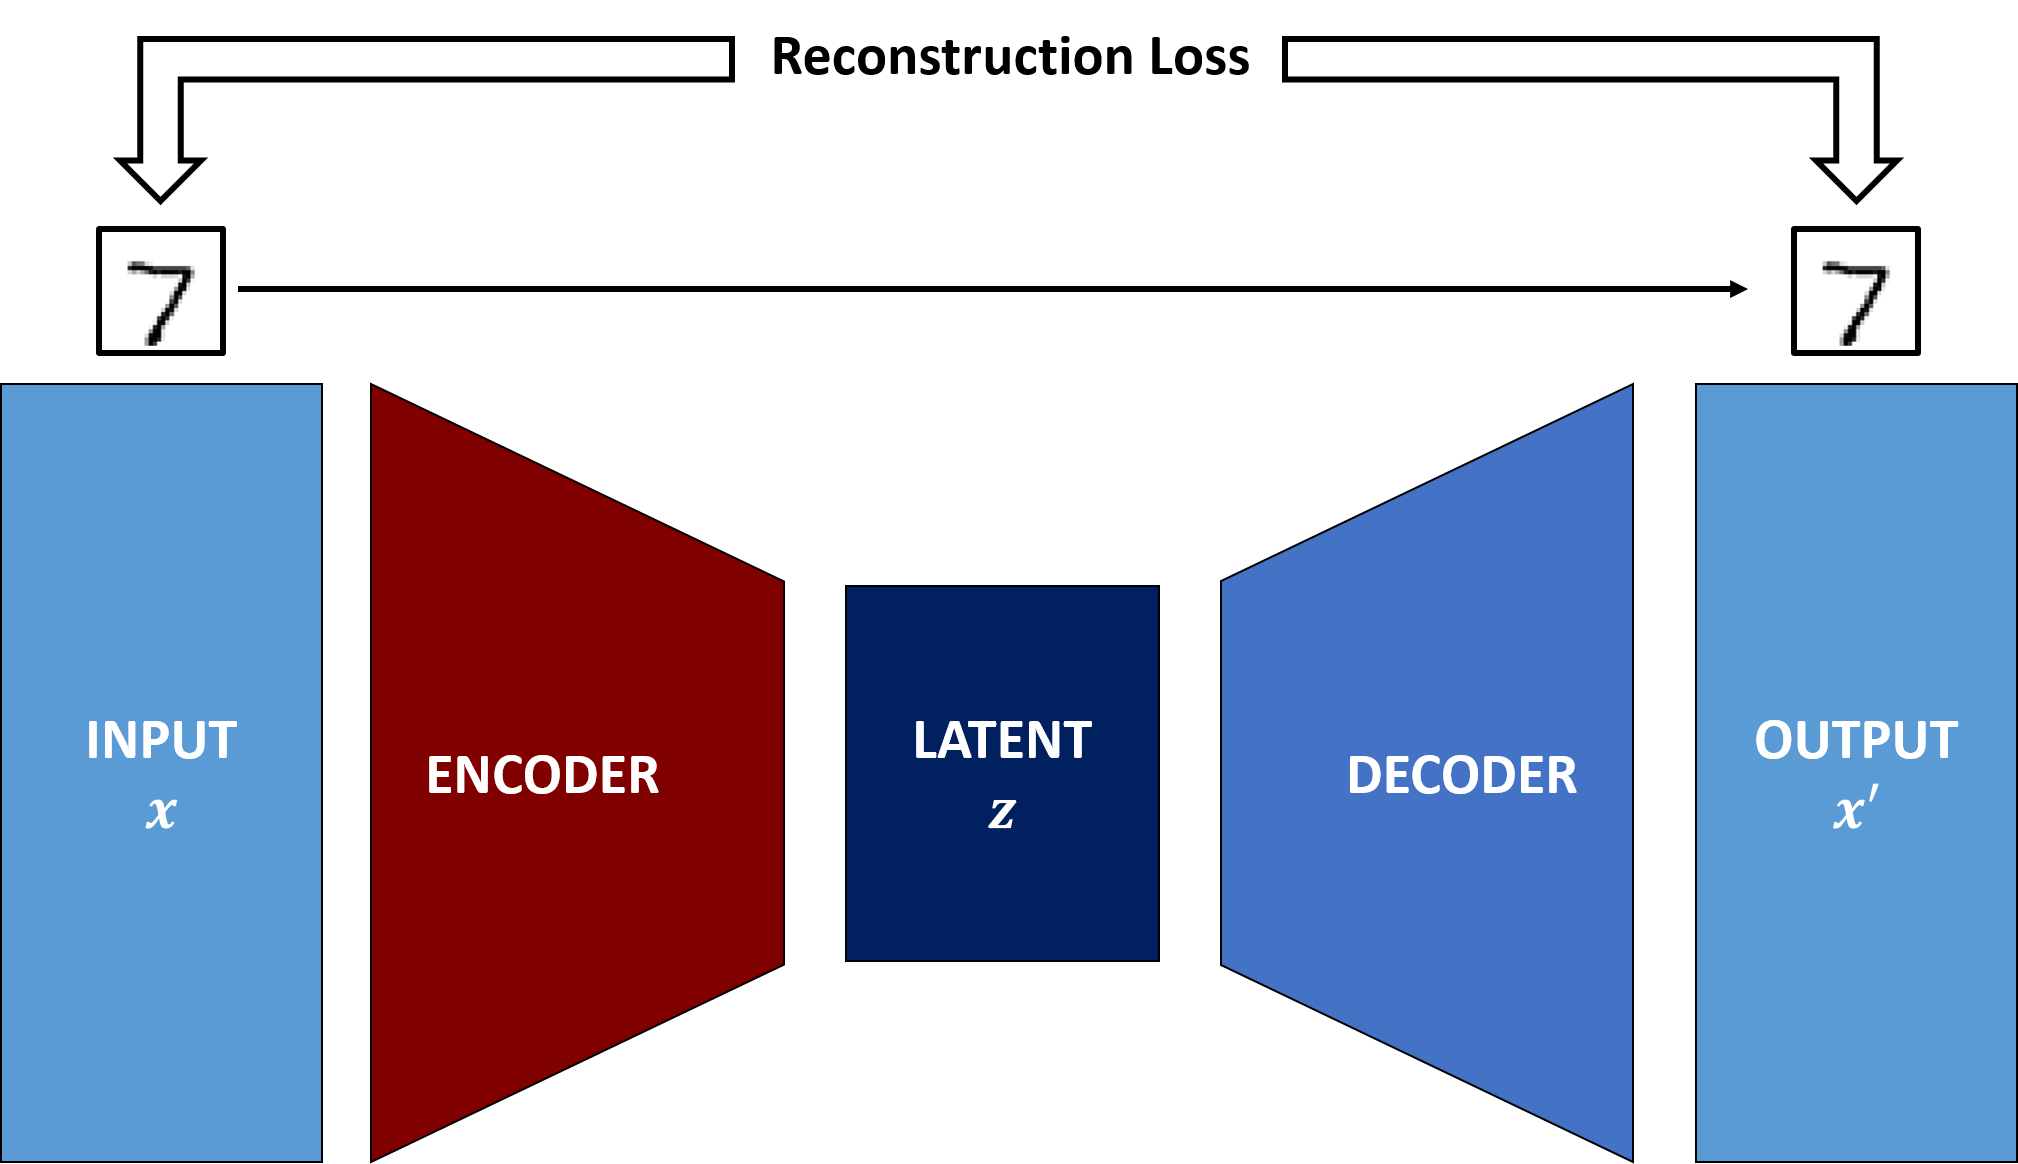
\includegraphics[width=0.5\textwidth]{imgs/autoencoder.png}
            \caption{Basic neural network structure of autoencoders}
            \label{fig:ae}
        \end{figure}
        
        There are many tasks autoencoders can achieve even in their basic form. The first is dimensionality reduction. If the dimension of the latent space is chosen to be less than that of the input space, then the autoencoder is forced to learn a compressed representation of the input space. In addition to the practical benefits, for example reducing the file size of images without losing too much quality, autoencoders perform a primitive form of feature learning.
        
        With a slight modification, autoencoders can also be used for image denoising. \cite{vincent2008extracting} proposed a denoising autoencoder which was able to remove noise from an image. This was achieved by first purposefully adding random noise from a fixed distribution to the original image and feeding the noisy image into the autoencoder. Then the autoencoder was trained by minimising the reconstruction loss between the final output image and the original (unaltered) image. As well as being able to remove noise from images, it was shown to be a more robust model and exhibited less overfitting than the original autoencoder.
        
        \begin{figure}[H]
            \centering
            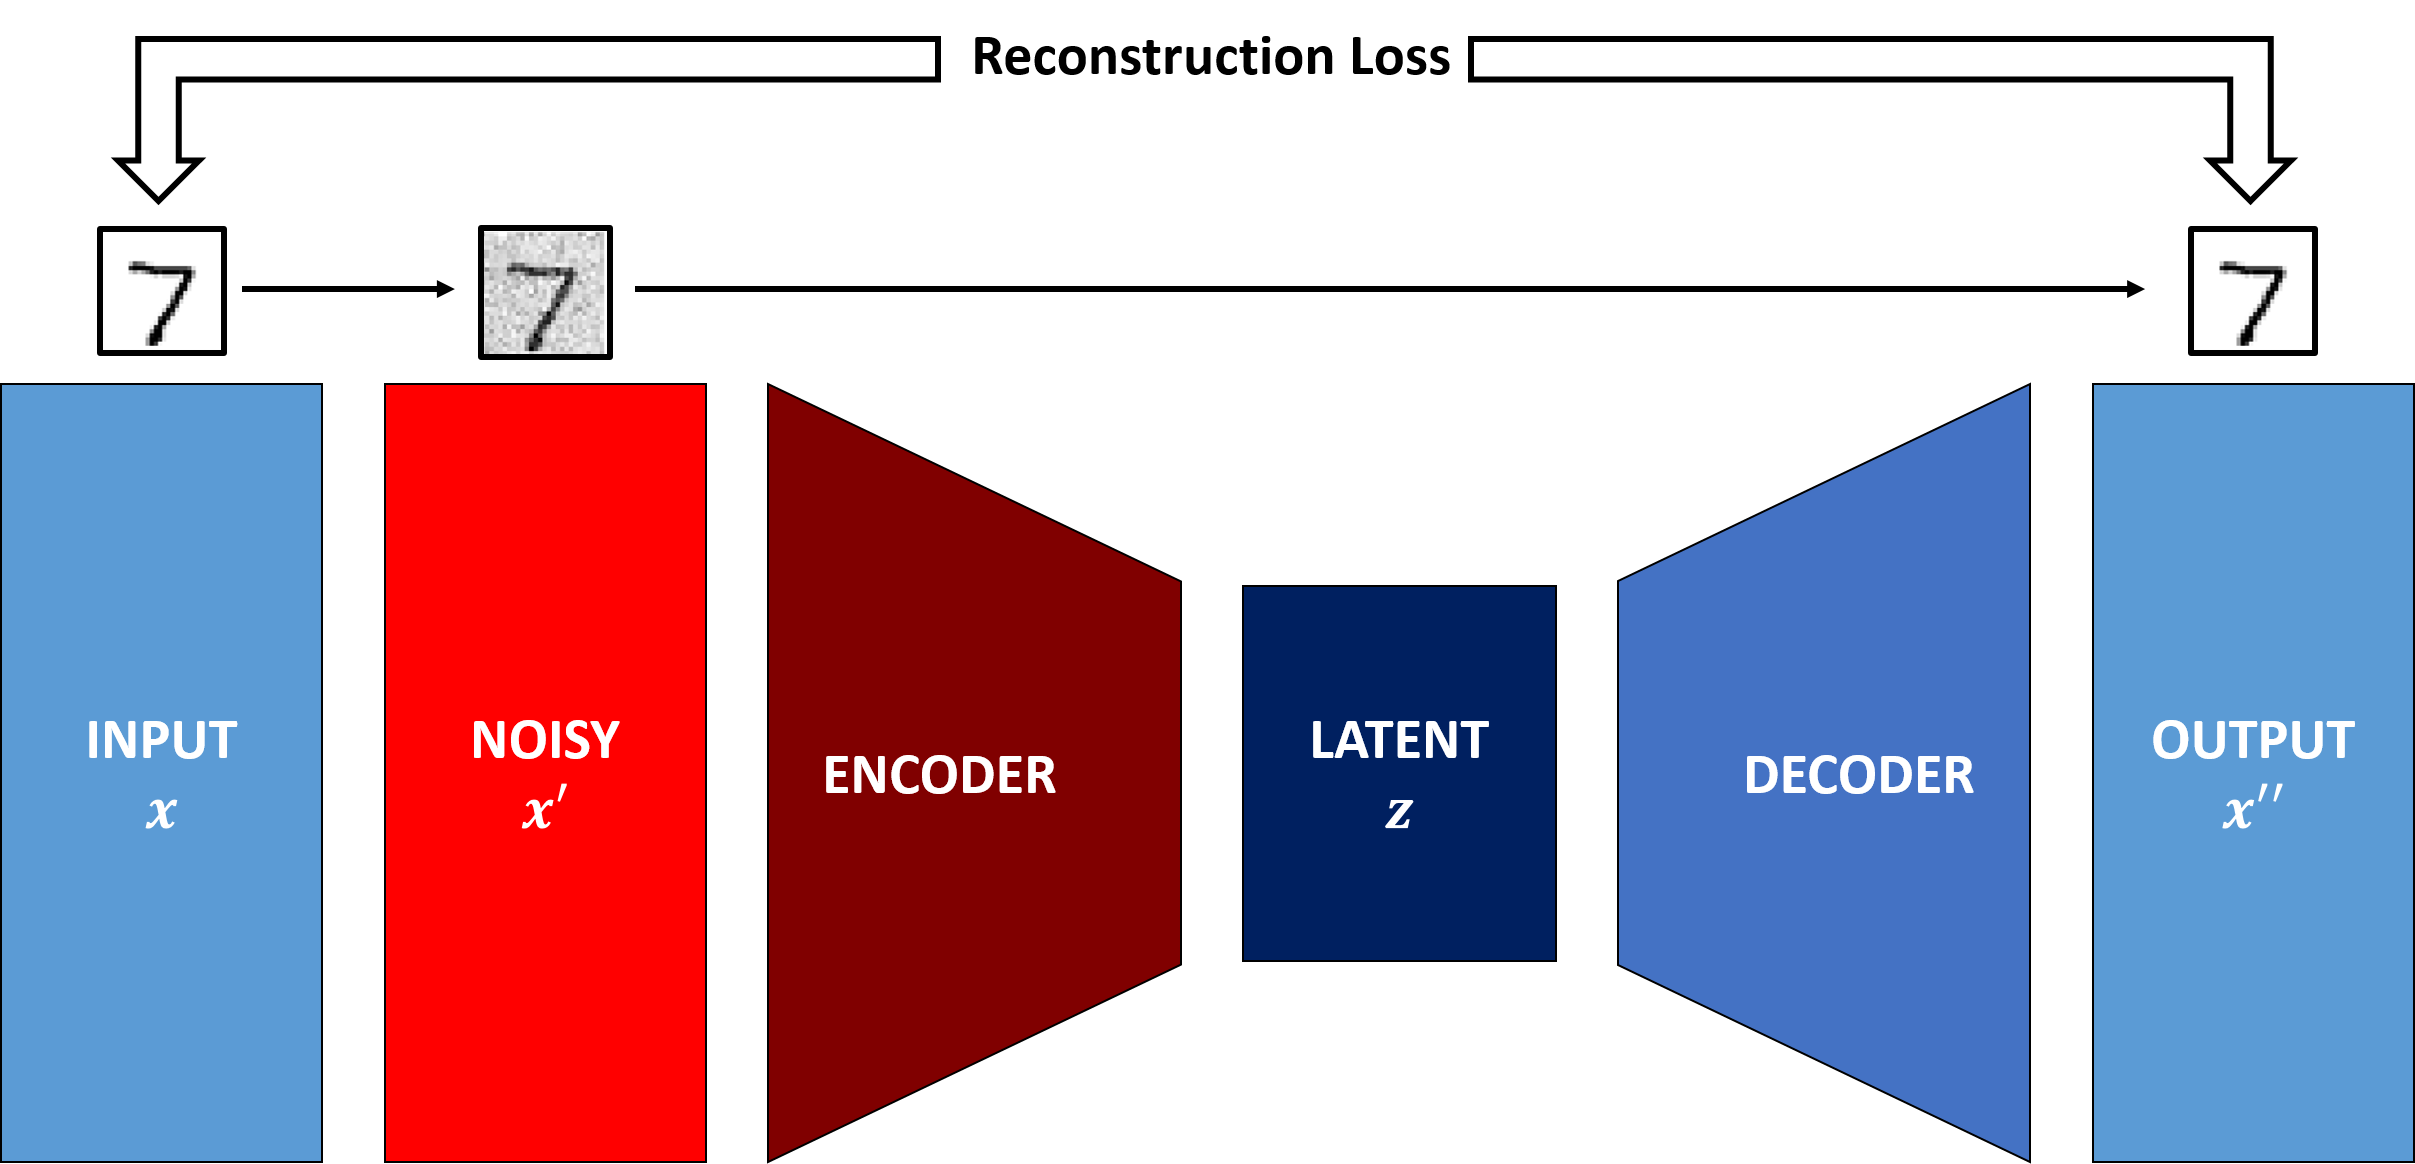
\includegraphics[width=0.5\textwidth]{imgs/denoising_ae.png}
            \caption{Structure of a denoising autoencoder neural network}
            \label{fig:dae}
        \end{figure}
        
        Autoencoders have been extended in many ways, such as Stacked Denoising Autoencoder \citep{vincent2010stacked}, Contractive Autoencoder \citep{rifai2011higher}, and k-Sparse Autoencoder \citep{makhzani2013k}. All of these approaches provided additional techniques for learning better performing models. However, basic autoencoders suffer from a fundamental limitation; they provided limited \textit{interpretability} of the latent space. There are two levels of interpretability we will discuss in this project: continuity in the latent space, and disentangled representations. These concepts are discussed further in the following sections.
        
    \section{Variational Autoencoder(VAE)}
        \subsection{Motivation}
            The VAE \citep{kingma2013auto} improves interpretability of the latent space by incorporating an additional loss term. As mentioned in the previous section, one limitation of the basic autoencoders is that their latent spaces have poor interpretability. For example, suppose we have a trained a basic autoencoder on a set of MNIST images. If we encode two different images of the digit `1' and get the corresponding latent vectors $\bm{z_1}$ and $\bm{z_2}$, what would happen if we take the mean of the two latent vectors, call it $\bm{z_{avg}}$, and feed this vector into the decoder? In many of the basic autoencoders, it is likely to produce nonsensical output. This is because the autoencoder had not been encouraged to produce a continuous latent space in which the latent vectors in between the learnt latent vectors would interpolate in a meaningful way. Without this encouragement, the latent space is going to be sparse and composed of disjoint clusters that represent the training data. An important implication of this limitation is that it is very difficult to generate new images, let alone generating new images with specifiable features.
            
            \begin{figure}[H]
                \centering
                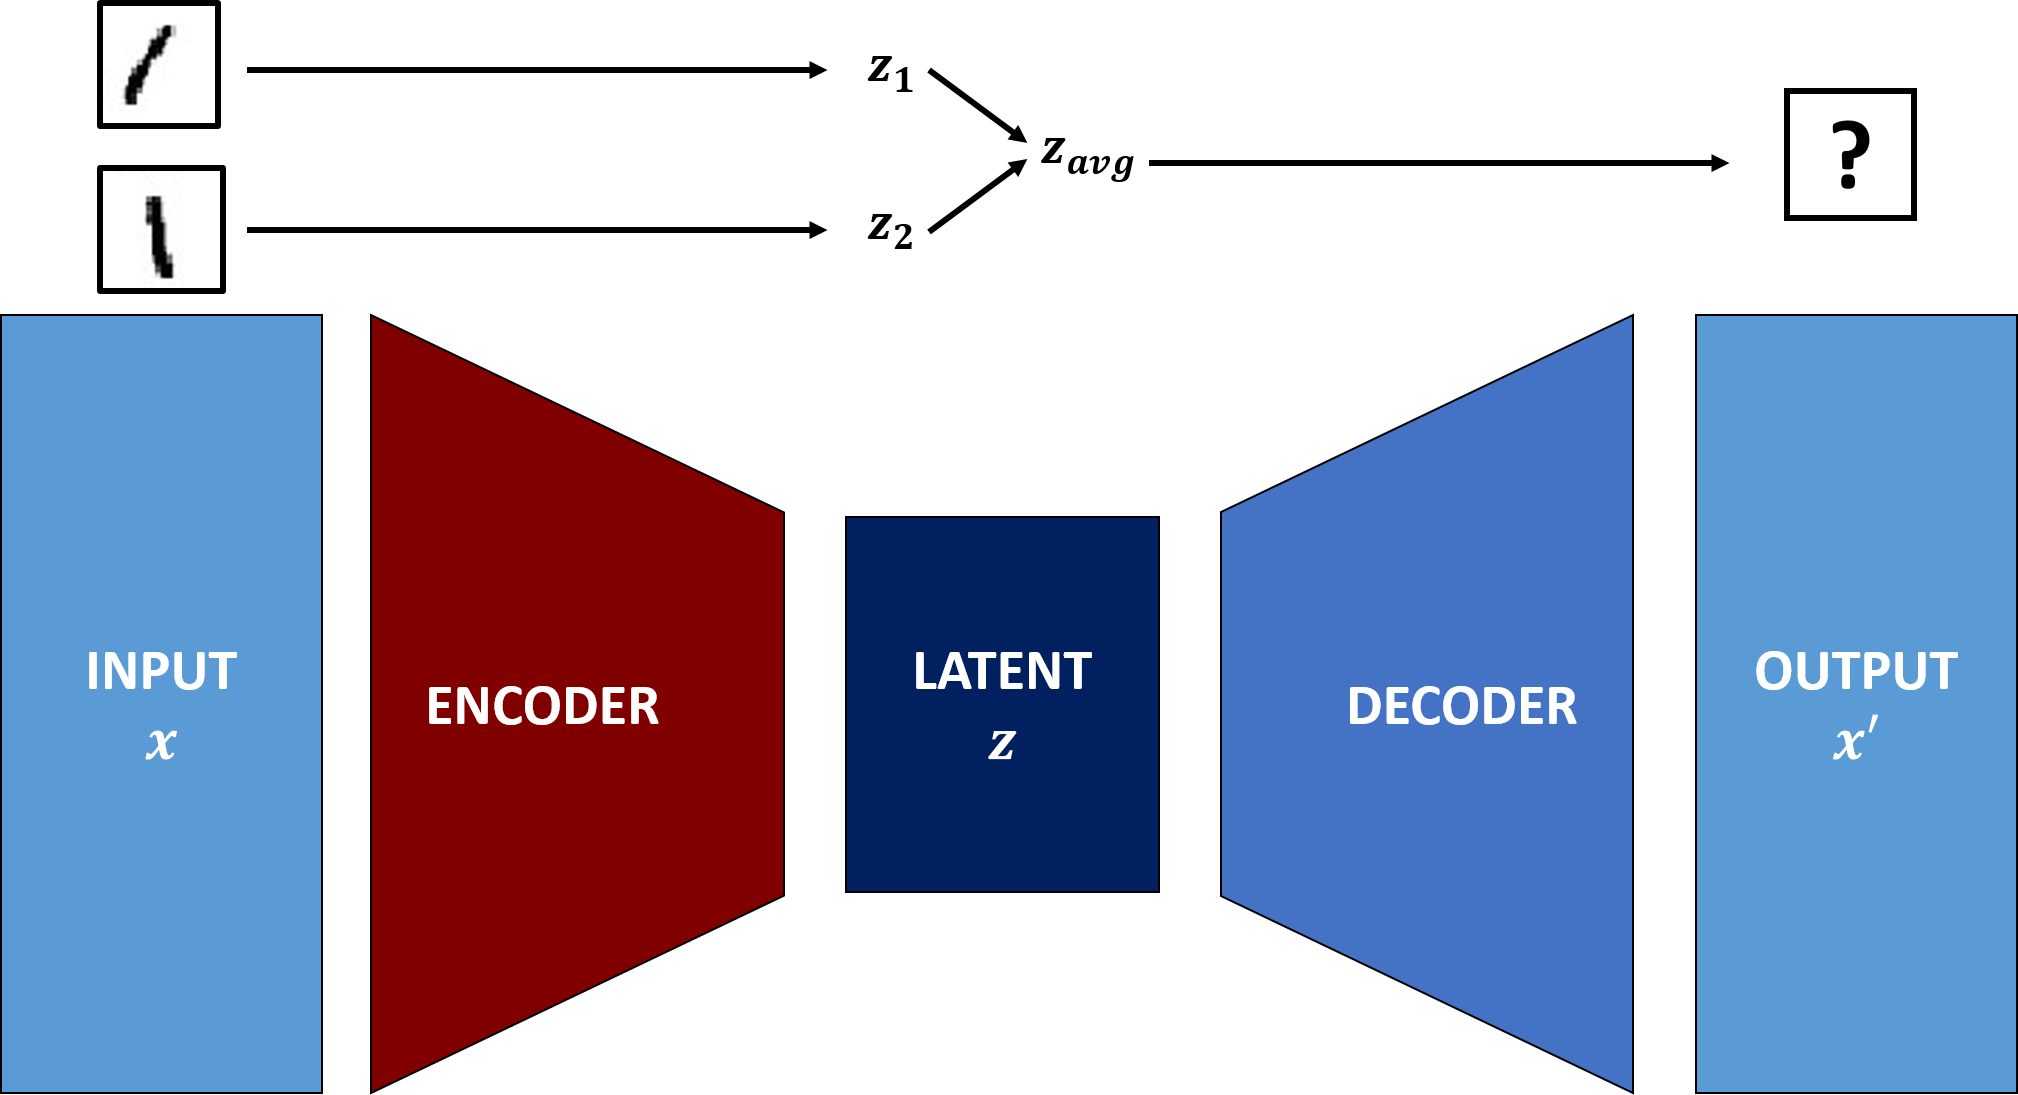
\includegraphics[width=0.5\textwidth]{imgs/interpolation_fail.png}
                \caption{Basic autoencoders have difficulty with interpolation}
                \label{fig:int_fail}
            \end{figure}
            
            On the other hand, VAEs produce a continuous latent space in which the interpolation between the latent vectors represent a much better interpolation between the original vectors. We will now discuss the theory behind the VAEs which makes this possible.
            
        \subsection{High level explanation of the VAE}
            VAE takes an input data point $\bm{x}$ and passes it through an encoder just like a basic autoencoder. However, instead of mapping the input data point as a latent data point, it maps it as a probability distribution $ENCODER(\bm{x}) \rightarrow q_{\bm{\theta_x}}(\bm{z}|\bm{x})$, where $\bm{\theta_x}$ is the parameter vector defining the distribution $q$. The standard distribution for the VAE's latent space is the uncorrelated multivariate Gaussian distribution $\mathcal{N}(\bm{\mu}, \bm{\Sigma})$ where $\bm{\Sigma}$ is a diagonal covariance matrix. So $\bm{\theta_x} = \{\bm{\mu_x}, \bm{\Sigma_x}\}$ and since $\bm{\Sigma_x}$ is diagonal, the mean $\mu_{x_i}$ and variance $\sigma_{x_i}^2$ in each dimension are all the parameters required to describe the distribution. This is the key which makes the meaningful continuous latent space possible as the VAE's latent space is composed of continuously overlapping distributions. From this distribution $q_{\bm{\theta_x}}(\bm{z}|\bm{x})$, a single latent vector is sampled at random $\bm{z'} \sim q_{\bm{\theta_x}}(\bm{z}|\bm{x})$ which is then fed into the decoder to construct the output vector $DECODER(\bm{z'}) \rightarrow \bm{x'}$.
            
            \begin{figure}[H]
                \centering
                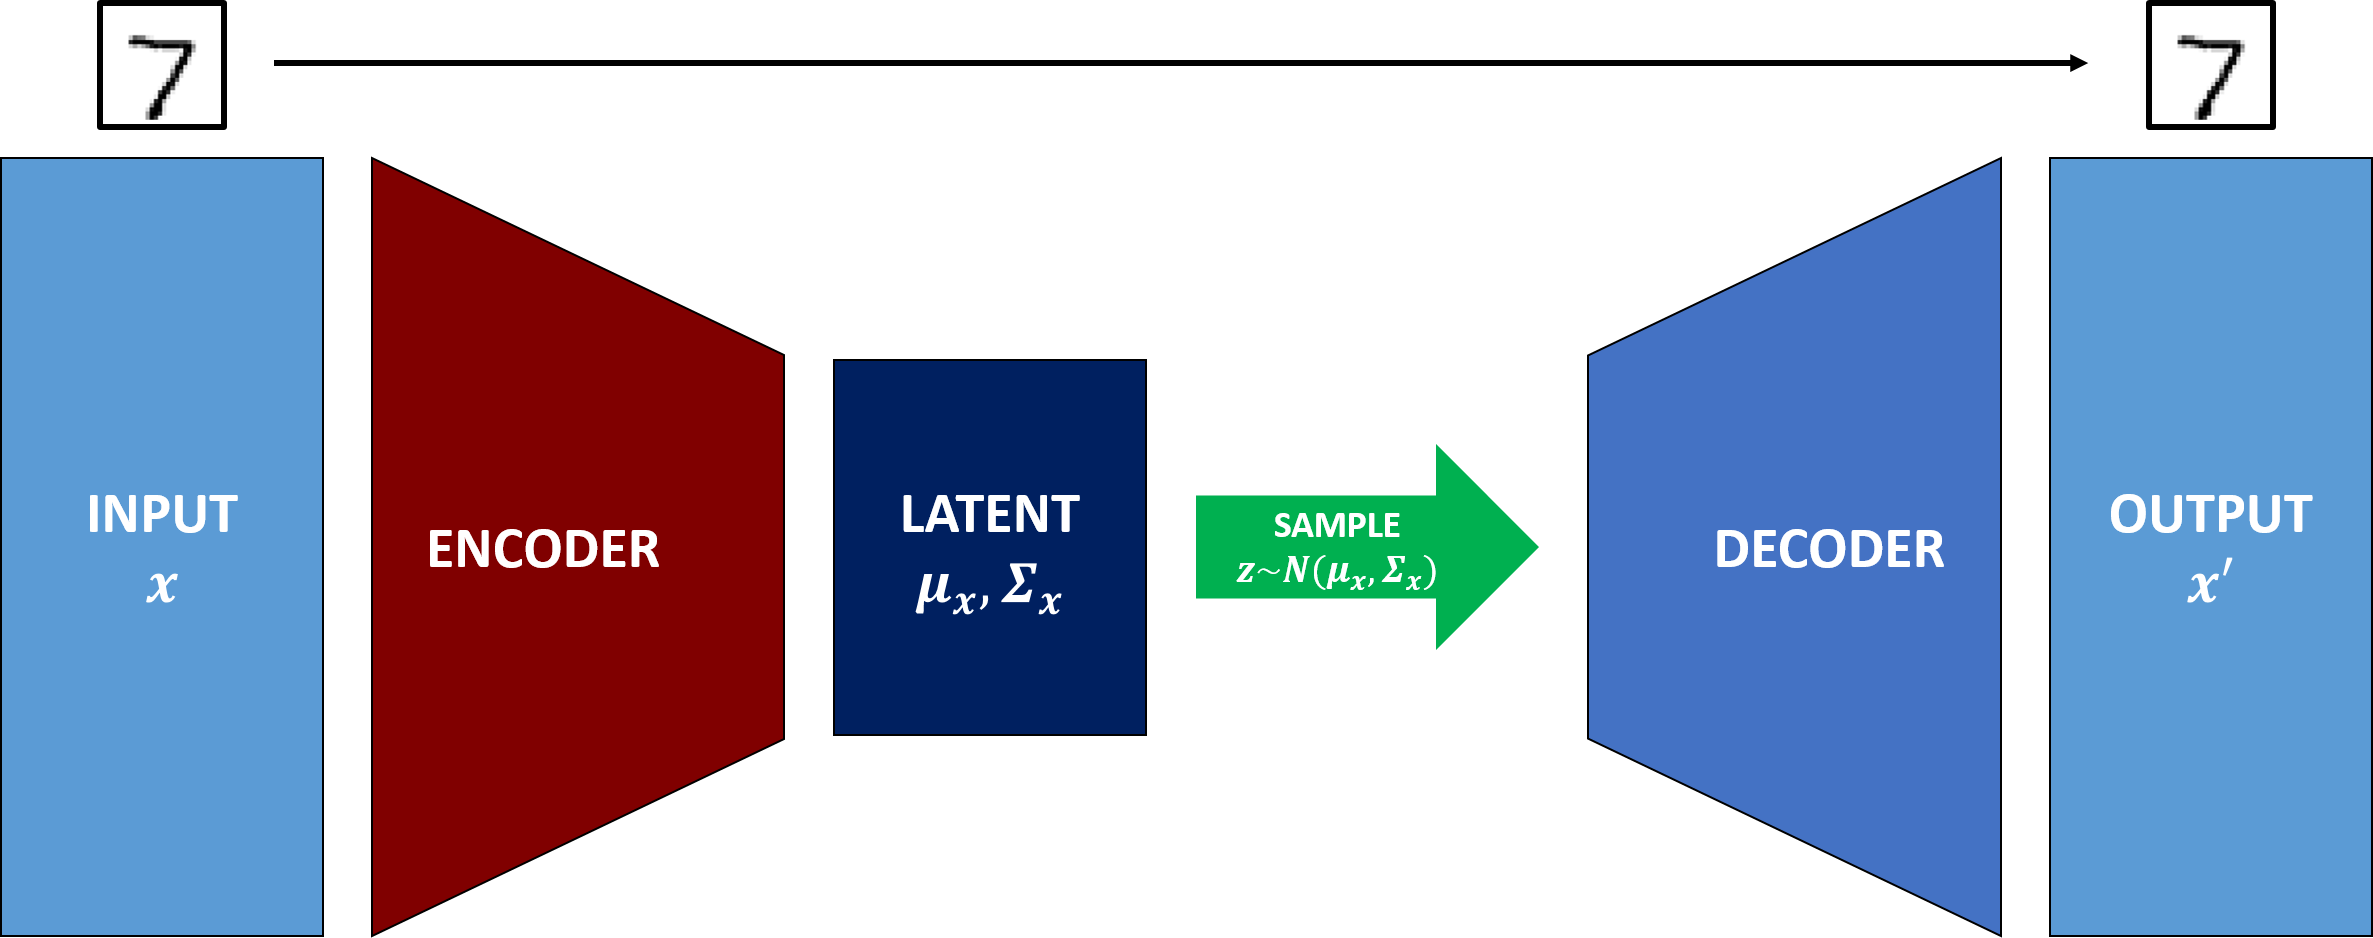
\includegraphics[width=0.5\textwidth]{imgs/vae_arch.png}
                \caption{VAE's architecture}
                \label{fig:vae_arch}
            \end{figure}

            When training a VAE, the process is slightly more involved. Firstly, since the latent features are distributions as opposed to single points, we cannot calculate the reconstruction loss in the same way as with basic autoencoders. What should the model compare the original input to? One possible candidate is the output of the mean of the encoded distribution. However, this approach will not be able to take the variance of the distribution into account. Another candidate is the output of a randomly sampled point from the encoded distribution. Unfortunately, a single point is insufficient to convey the information of the whole distribution. What we need is to take a large enough sample from the distribution and take the expectation of the reconstruction losses between the original input and the sampled outputs.
            
            \begin{figure}[H]
                \centering
                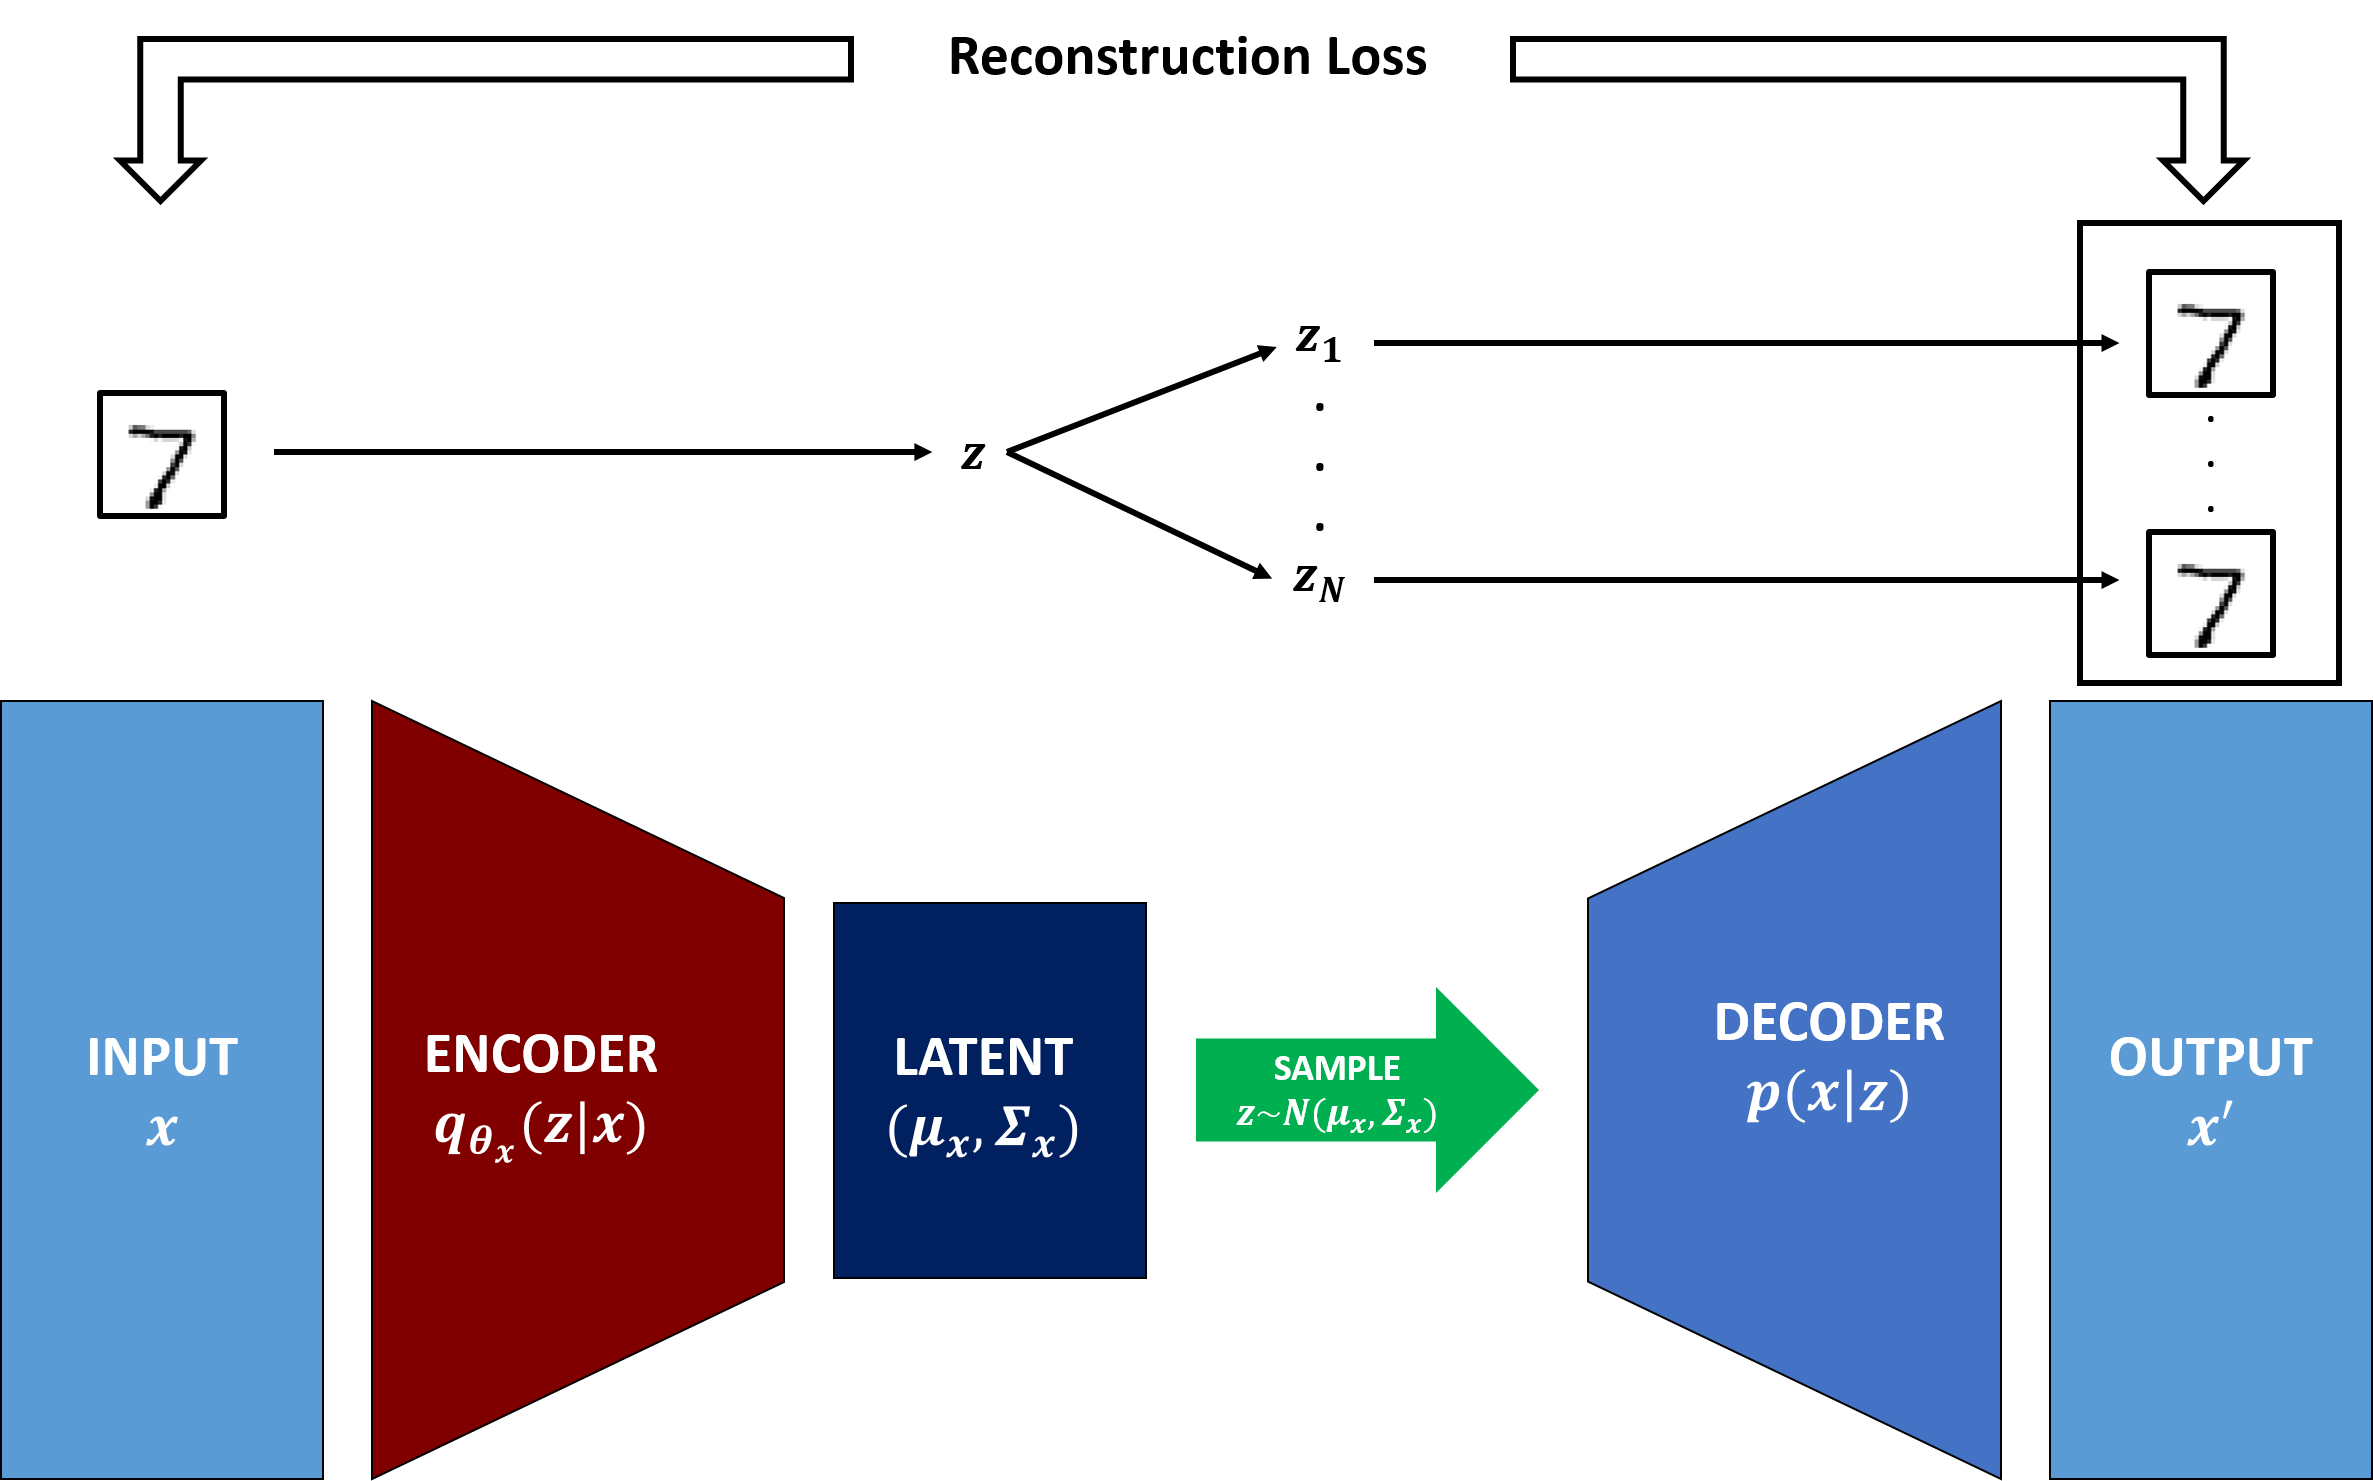
\includegraphics[width=0.5\textwidth]{imgs/recon_loss.png}
                \caption{VAE's reconstruction loss}
                \label{fig:recon_loss}
            \end{figure}
            
            So far, what we have is a model which will learn to best represent the input space by modelling the latent space with Gaussian distributions. However, there is nothing stopping the model from using of all of the dimensions in the latent space and produce many disjoint Gaussians with very small variances. This issue is magnified if the dimension of the latent space is much larger than the number of features present in the input space. The consequence of this overfitting is that the model does not learn a continuous latent space. Instead, the model learns disjoint clusters which vary across the various dimensions. To combat this issue, the standard loss function is expanded to include a regulariser which penalises the model for using more dimensions that necessary as well as using Gaussians with small variance.  The Kullback–Leibler divergence \citep{kullback1951information}(KL divergence) is used to quantify the penalty. The exact mathematical definition and the derivation of the KL divergence's appearance in the loss function is discussed below, but for now, we will simply explain what effect the KL divergence has on the model. KL divergence is like a metric which measures the difference between two probability distributions. With this, we will measure the difference between $q_{\bm{\theta}}(\bm{z}|\bm{x}_{in})$ and $p(\bm{z})$ where $p(\bm{z})$ is the standard Gaussian distribution $\mathcal{N}(\bm{0}, \bm{I})$. Now if we add this KL divergence term to our loss, the model is pushed to keep the shape of $q_{\bm{\theta}}(\bm{z}|\bm{x}_{in})$ similar to a standard Gaussian, otherwise KL divergence will become large and incur a large loss. This has two main implications. First, VAE will try to keep as much latent dimensions to have standard Gaussian parameters which leads to using the least number of latent dimensions as possible. Secondly, VAE will be penalised when it tries to use small standard deviations to create small size clusters. This means that VAE is encouraged to cluster of a larger number of data points together, which results in a larger number of nearby data points being mapped to the same distribution. This will be explained in more detail in \ref{subsec:beta_reasoning}.
            
            In summary, VAE is trained with the sum of the reconstruction loss, which is the expectation of the differences between the original input data and the samples of output data, together with the KL divergence between the latent uncorrelated Gaussian distribution and the standard Gaussian distribution:
            \begin{equation}
                \text{Loss\textsubscript{VAE}} = \text{Reconstruction Loss} + \text{KL Divergence}
                \label{eqn:loss_vae}
            \end{equation}
            
        \subsection{Probabilistic descriptions and mathematical derivations}
            We start with the observed space $\bm{X}$ composed of data points $\bm{x}$. We begin with an assumption that the each $\bm{x}$ are independently and identically distributed(iid) by some probability function of some corresponding latent variables $\bm{z}$ which are unobserved or hidden. Let $p(\bm{x}|\bm{z})$ be the probability of observing $\bm{x}$ given the latent $\bm{z}$, also known as the \textit{likelihood} function. We also assume that each latent $\bm{z}$ are distributed with some function which we denote by $p(\bm{z})$, also known as the \textit{prior}. The relationship can be illustrated with the following graphical model:
            
            \begin{figure}[H]
                \centering
                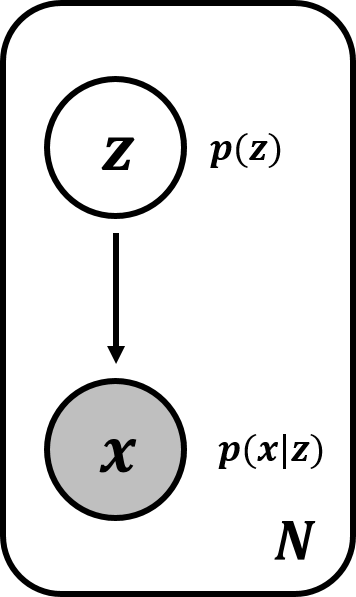
\includegraphics[width=0.15\textwidth]{imgs/x_z_graph.png}
                \caption{The graphical model showing the relationship between $\bm{x}$ and $\bm{z}$}
                \label{fig:x_z_graph}
            \end{figure}
            
            Now given the prior and the likelihood, we can use the classical Bayes' theorem to express the \textit{posterior}:
            
            \begin{align*} 
                p(\bm{z}|\bm{x}) &= \frac{p(\bm{z},\bm{x})}{p(\bm{x})}\\
                &= \frac{p(\bm{x} | \bm{z})p(\bm{z})}{p(\bm{x})}\\
                &= \frac{p(\bm{x} | \bm{z})p(\bm{z})}{\int p(\bm{x}, \bm{z}) dz}\\
                &= \frac{p(\bm{x} | \bm{z})p(\bm{z})}{\int p(\bm{x} | \bm{z}) p(\bm{z}) dz}\\
            \end{align*}

            Unfortunately, the term which appears in the denominator of the posterior: $p(\bm{x}) = \int p(\bm{x} | \bm{z}) p(\bm{z}) dz$, is intractable as the integral requires exponential computational time to calculate over all the possible values of the latents. Because of this problem of intractable posterior, VAE instead uses a family of tractable functions $q_{\bm{\theta_x}}(\bm{z}|\bm{x})$ which best \textit{approximates} the true posterior $p(\bm{z}|\bm{x})$. Notice that the family of functions are parametrised by $\bm{\theta_x}$ which in turn depends on the input $\bm{x}$. In the standard VAE, $q_{\bm{\theta}}(\bm{z}|\bm{x})$ are chosen to be Gaussians which means that $\bm{\theta_x}= \{\bm{\mu_x}, \bm{\Sigma_x}\}$.
            
            Now in order to make sure that $q_{\bm{\theta_x}}(\bm{z}|\bm{x})$ closely approximates $p(\bm{z}|\bm{x})$, we can minimise:
                \[ KL\left[q_{\bm{\theta_x}}(\bm{z}|\bm{x}) || p(\bm{z}|\bm{x})\right] \]
            where the $KL\left[q(\bm{x}) || p(\bm{x})\right]$ is the Kullback-Leibler(KL) divergence, measuring the difference between the two distributions, defined by:
                \[ KL\left[q(\bm{x}) || p(\bm{x})\right] := \int_{\bm{x} \in \bm{X}} q(\bm{x}) \log \frac{q(\bm{x})}{p(\bm{x})} d\bm{x}\]
            In other words, we wish to minimise:
                \[ KL\left[q_{\bm{\theta_x}}(\bm{z}|\bm{x}) || p(\bm{z}|\bm{x})\right] = \int_{\bm{z} \in \bm{Z}} q_{\bm{\theta_x}}(\bm{z}|\bm{x}) \log \frac{q_{\bm{\theta_x}}(\bm{z}|\bm{x})}{p(\bm{z}|\bm{x})} d\bm{z}\]
            
            The problem is not yet solved as the term still includes the intractable posterior $p(\bm{z}|\bm{x})$. To address this problem, we will minimise the KL divergence indirectly by using what's known as the \textit{Evidence Lower BOund}($ELBO$):
                \[ ELBO(\bm{\theta_x}) := \log p(\bm{x}) - KL\left[q_{\bm{\theta_x}}(\bm{z}|\bm{x}) || p(\bm{z}|\bm{x})\right] \]
            Keeping all other parameters fixed, we can see that maximising $ELBO$ with respect to $\bm{\theta_x}$ minimises the KL divergence since the KL divergence is non-negative due to Jensen's inequality\citep{jensen1906fonctions}. Doing some algebraic manipulation removes both intractable terms $p(\bm{x})$ and $p(\bm{z}|\bm{x})$ in the equation. We first begin by manipulating $\log p(\bm{x})$:
            
            \begin{align*}
              \log p(\bm{x}) &= \log p(\bm{x}) \int_{\bm{z} \in \bm{Z}} q_{\bm{\theta_x}}(\bm{z}|\bm{x}) d\bm{z} & \text{$q$ is a probability density function}\\
                &= \int_{\bm{z} \in \bm{Z}} q_{\bm{\theta_x}}(\bm{z}|\bm{x}) \log p(\bm{x}) d\bm{z} & \text{$\bm{z}$ does not appear in $\log p(\bm{x})$}\\
                &= \int_{\bm{z} \in \bm{Z}} q_{\bm{\theta_x}}(\bm{z}|\bm{x}) \log \frac{p(\bm{x}, \bm{z})}{p(\bm{z} | \bm{x})} d\bm{z} & \text{Using $p(\bm{z} | \bm{x}) = \frac{p(\bm{x}, \bm{z})}{p(\bm{x})}$}\\
                &= \int_{\bm{z} \in \bm{Z}} q_{\bm{\theta_x}}(\bm{z}|\bm{x}) \log \frac{p(\bm{x}, \bm{z})}{q_{\bm{\theta_x}}(\bm{z}|\bm{x})}\frac{q_{\bm{\theta_x}}(\bm{z}|\bm{x})}{p(\bm{z} | \bm{x})} d\bm{z} & \frac{q_{\bm{\theta_x}}(\bm{z}|\bm{x})}{q_{\bm{\theta_x}}(\bm{z}|\bm{x})} = 1\\
                &= \int_{\bm{z} \in \bm{Z}} q_{\bm{\theta_x}}(\bm{z}|\bm{x}) \log \frac{p(\bm{x}, \bm{z})}{q_{\bm{\theta_x}}(\bm{z}|\bm{x})} + q_{\bm{\theta_x}}(\bm{z}|\bm{x}) \log \frac{q_{\bm{\theta_x}}(\bm{z}|\bm{x})}{p(\bm{z} | \bm{x})} d\bm{z} & \text{$\log$ property}\\
                &= \int_{\bm{z} \in \bm{Z}} q_{\bm{\theta_x}}(\bm{z}|\bm{x}) \log \frac{p(\bm{x}, \bm{z})}{q_{\bm{\theta_x}}(\bm{z}|\bm{x})} d\bm{z} + \int_{\bm{z} \in \bm{Z}} q_{\bm{\theta_x}}(\bm{z}|\bm{x}) \log \frac{q_{\bm{\theta_x}}(\bm{z}|\bm{x})}{p(\bm{z} | \bm{x})} d\bm{z} & \text{Linearity of integrals}\\
                &= \int_{\bm{z} \in \bm{Z}} q_{\bm{\theta_x}}(\bm{z}|\bm{x}) \log \frac{p(\bm{x}, \bm{z})}{q_{\bm{\theta_x}}(\bm{z}|\bm{x})}d\bm{z} + KL\left[q_{\bm{\theta_x}}(\bm{z}|\bm{x}) || p(\bm{z}|\bm{x})\right] & \text{Definition of $KL$}\\
            \end{align*}
            
            Therefore, substituting the final form back into $ELBO$, we get:
            
            \begin{align*}
                ELBO(\bm{\theta_x}) &= \log p(\bm{x}) - KL\left[q_{\bm{\theta_x}}(\bm{z}|\bm{x}) || p(\bm{z}|\bm{x})\right]\\
                &= \int_{\bm{z} \in \bm{Z}} q_{\bm{\theta_x}}(\bm{z}|\bm{x}) \log \frac{p(\bm{x}, \bm{z})}{q_{\bm{\theta_x}}(\bm{z}|\bm{x})} d\bm{z} + KL\left[q_{\bm{\theta_x}}(\bm{z}|\bm{x}) || p(\bm{z}|\bm{x})\right] - KL\left[q_{\bm{\theta_x}}(\bm{z}|\bm{x}) || p(\bm{z}|\bm{x})\right]\\
                &= \int_{\bm{z} \in \bm{Z}} q_{\bm{\theta_x}}(\bm{z}|\bm{x}) \log \frac{p(\bm{x}, \bm{z})}{q_{\bm{\theta_x}}(\bm{z}|\bm{x})} d\bm{z}\\
                &= \int_{\bm{z} \in \bm{Z}} q_{\bm{\theta_x}}(\bm{z}|\bm{x}) \log \frac{p(\bm{x} | \bm{z})p(\bm{z})}{q_{\bm{\theta_x}}(\bm{z}|\bm{x})} d\bm{z}\\
                &= \int_{\bm{z} \in \bm{Z}} q_{\bm{\theta_x}}(\bm{z}|\bm{x}) \log p(\bm{x} | \bm{z}) + q_{\bm{\theta_x}}(\bm{z}|\bm{x}) \log \frac{p(\bm{z})}{q_{\bm{\theta_x}}(\bm{z}|\bm{x})} d\bm{z}\\
                &= \int_{\bm{z} \in \bm{Z}} q_{\bm{\theta_x}}(\bm{z}|\bm{x}) \log p(\bm{x} | \bm{z}) d\bm{z} + \int_{\bm{z} \in \bm{Z}} q_{\bm{\theta_x}}(\bm{z}|\bm{x}) \log \frac{p(\bm{z})}{q_{\bm{\theta_x}}(\bm{z}|\bm{x})} d\bm{z}\\
                &= \mathbb{E}_{q_{\bm{\theta_x}}(\bm{z}|\bm{x})} \left[\log p(\bm{x} | \bm{z}) \right] + KL\left[q_{\bm{\theta_x}}(\bm{z}|\bm{x}) || p(\bm{z})\right]\\
            \end{align*}
            
            As claimed above, all terms in this expression are tractable and so we can use $ELBO$ as our loss function. We also notice that this is exactly what we had in \ref{eqn:loss_vae}:
            
            \[ \boxed{\text{Loss\textsubscript{VAE}} = \underbrace{\mathbb{E}_{q_{\bm{\theta_x}}(\bm{z}|\bm{x})} \left[\log p(\bm{x} | \bm{z}) \right]}_\textrm{Reconstruction Loss} + \underbrace{KL\left[q_{\bm{\theta_x}}(\bm{z}|\bm{x}) || p(\bm{z})\right]}_\textrm{KL Divergence}} \]
            
        \subsection{The reparametrisation trick}
            There is one last difficulty that must be addressed in implementing the VAE as a neural network. In \ref{fig:vae_arch}, one of the operation in the network is sampling from the latent distribution:
            
            \begin{figure}[H]
                \centering
                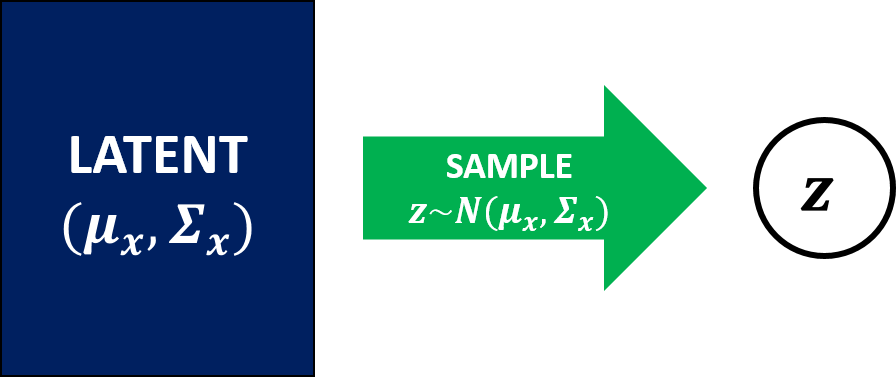
\includegraphics[width=0.4\textwidth]{imgs/sampling.png}
                \caption{We cannot back propagate through sampling}
                \label{fig:sampling}
            \end{figure}
            
            Unfortunately, sampling is not an operation in which we can take the gradient for back propagation. To deal with this problem, \cite{kingma2013auto} takes advantage of the fact that the covariance $\bm{\Sigma_x}$ is a diagonal matrix and use a technique called \textit{the reparametrisation trick} in which we arrive at the sampled latent $\bm{z}$ not directly from the latent Gaussian distribution, but indirectly by sampling a noise vector from a standard Gaussian distribution and then arriving at the latent $\bm{z}$ by scaling it by $\bm{\Sigma_x}$ and by translating it by $\bm{\mu_x}$. This has the same output as sampling directly from the latent distribution but now at least we can take the separate gradient through $\frac{\partial \bm{z}}{\partial \bm{\mu_x}}$ and $\frac{\partial \bm{z}}{\partial \bm{\Sigma_x}}$:
            
            \begin{figure}[H]
                \centering
                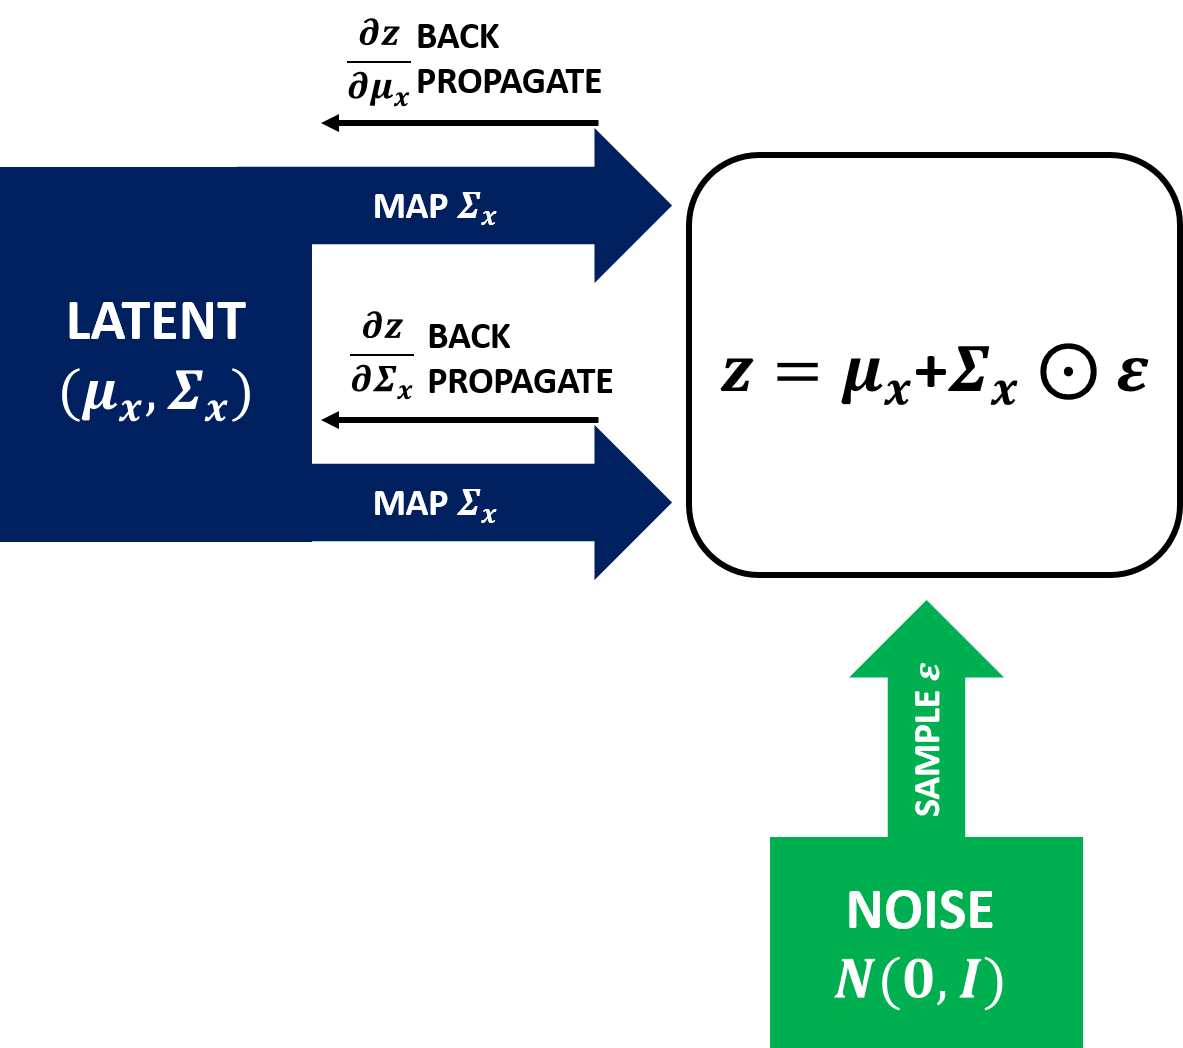
\includegraphics[width=0.4\textwidth]{imgs/reparametrisation_trick.png}
                \caption{The reparametrisation trick}
                \label{fig:reparametrisation_trick}
            \end{figure}
            
            So the actual full architecture of VAE is the following.
            
            \begin{figure}[H]
                \centering
                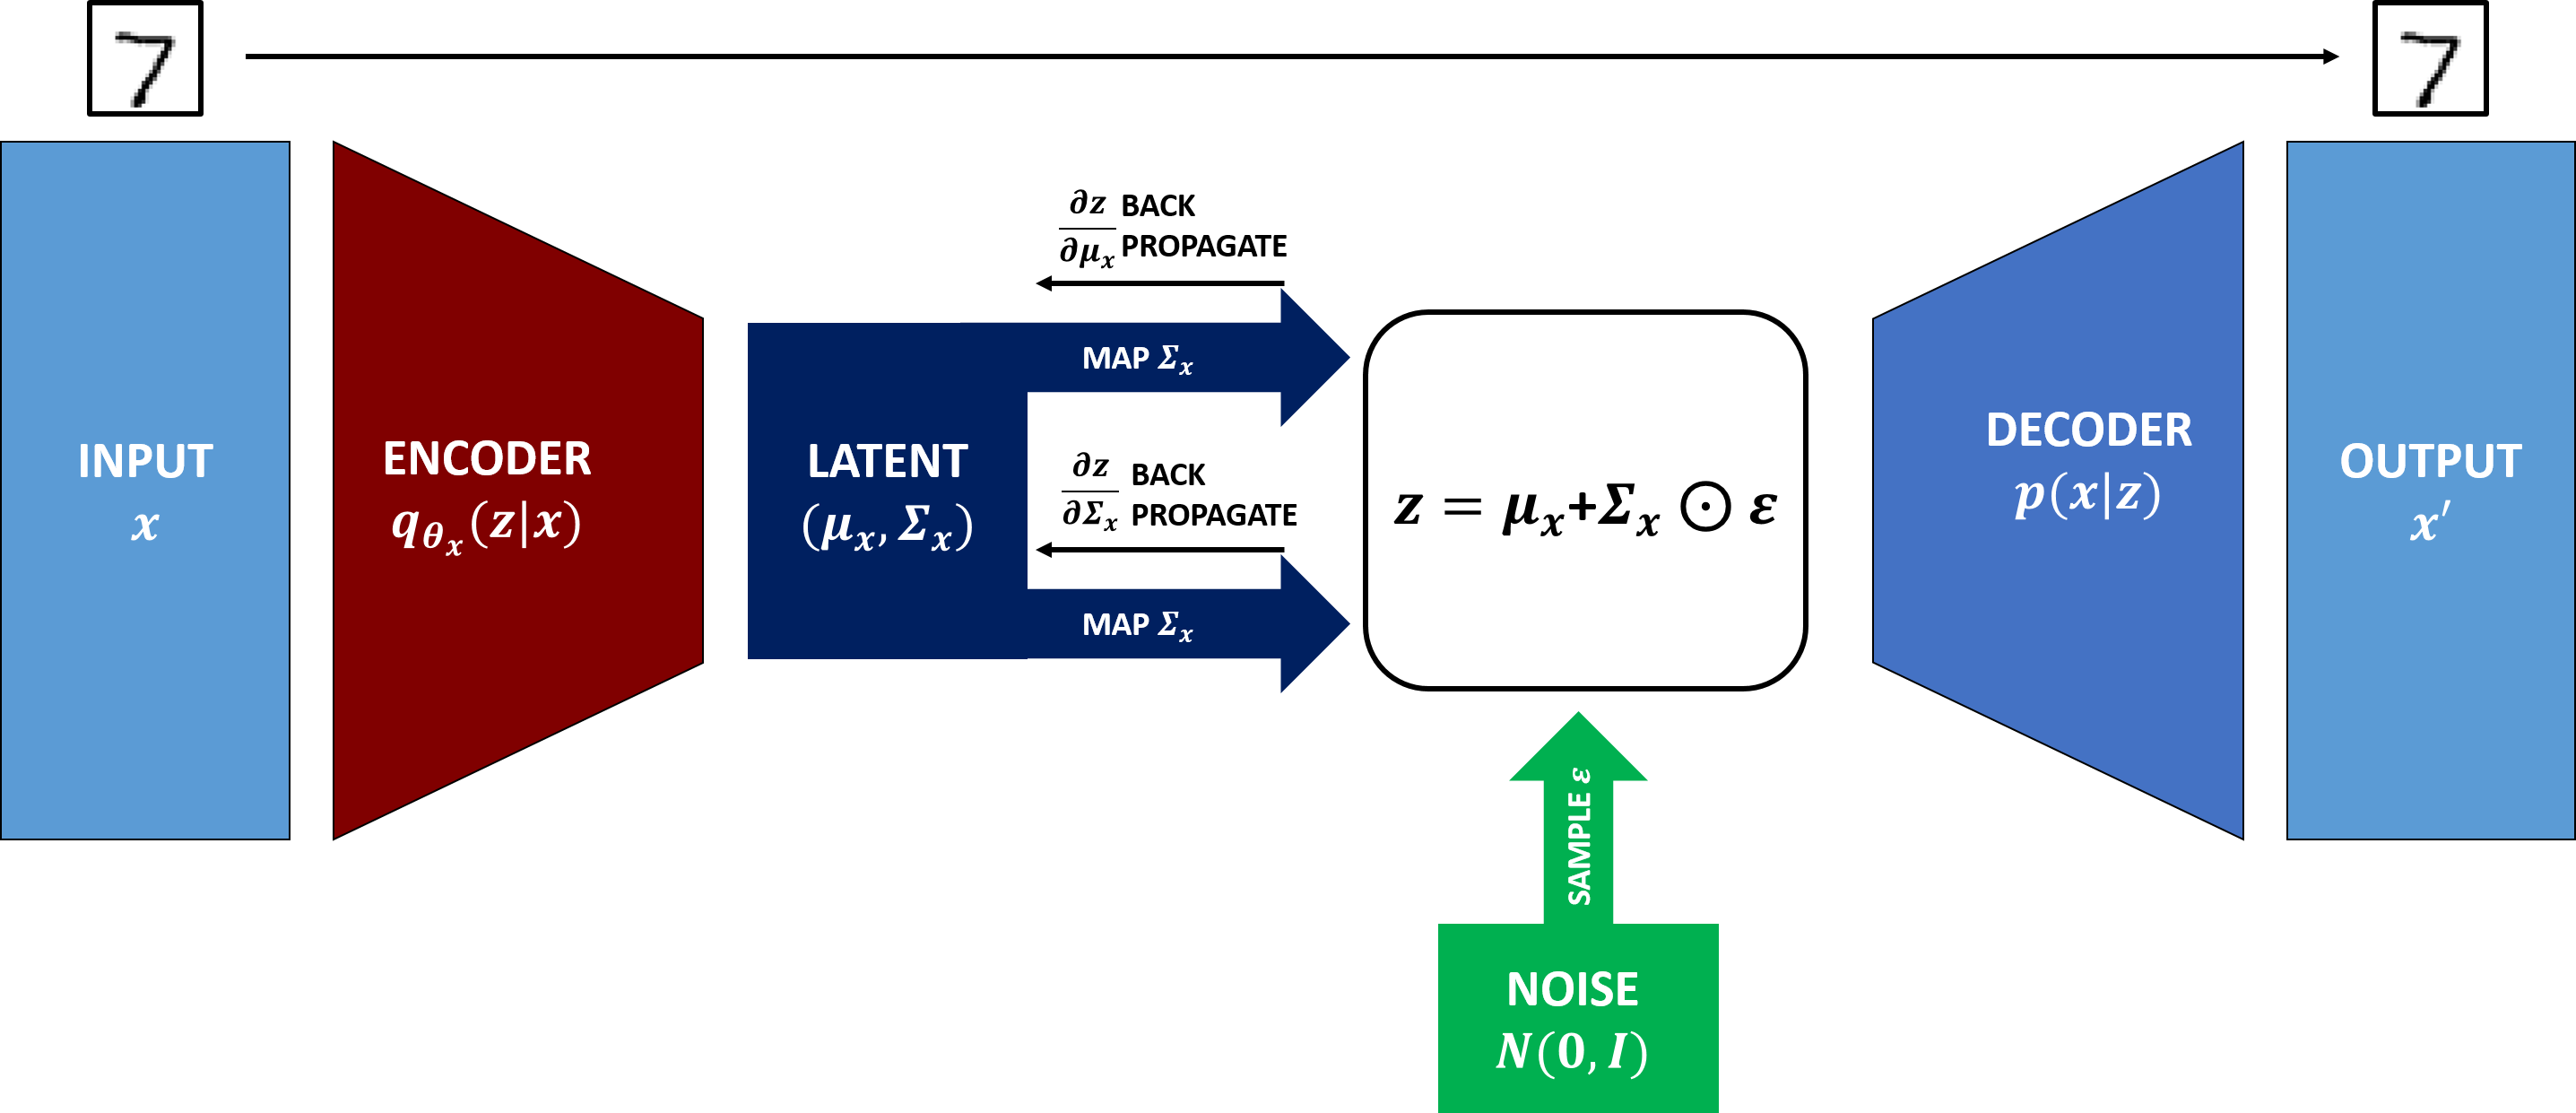
\includegraphics[width=1\textwidth]{imgs/vae_arch2.png}
                \caption{The full VAE architecture}
                \label{fig:vae_arch2}
            \end{figure}
            
        \subsection{Outputs}
            \cite{kingma2013auto} already showed that VAE produces latent spaces which satisfy our first condition of interpretability very well: it produces a continuous latent space in which locality in the input space is preserved in the latent space which allows for great interpolations between data points.
            
            \begin{figure}[H]
                \centering
                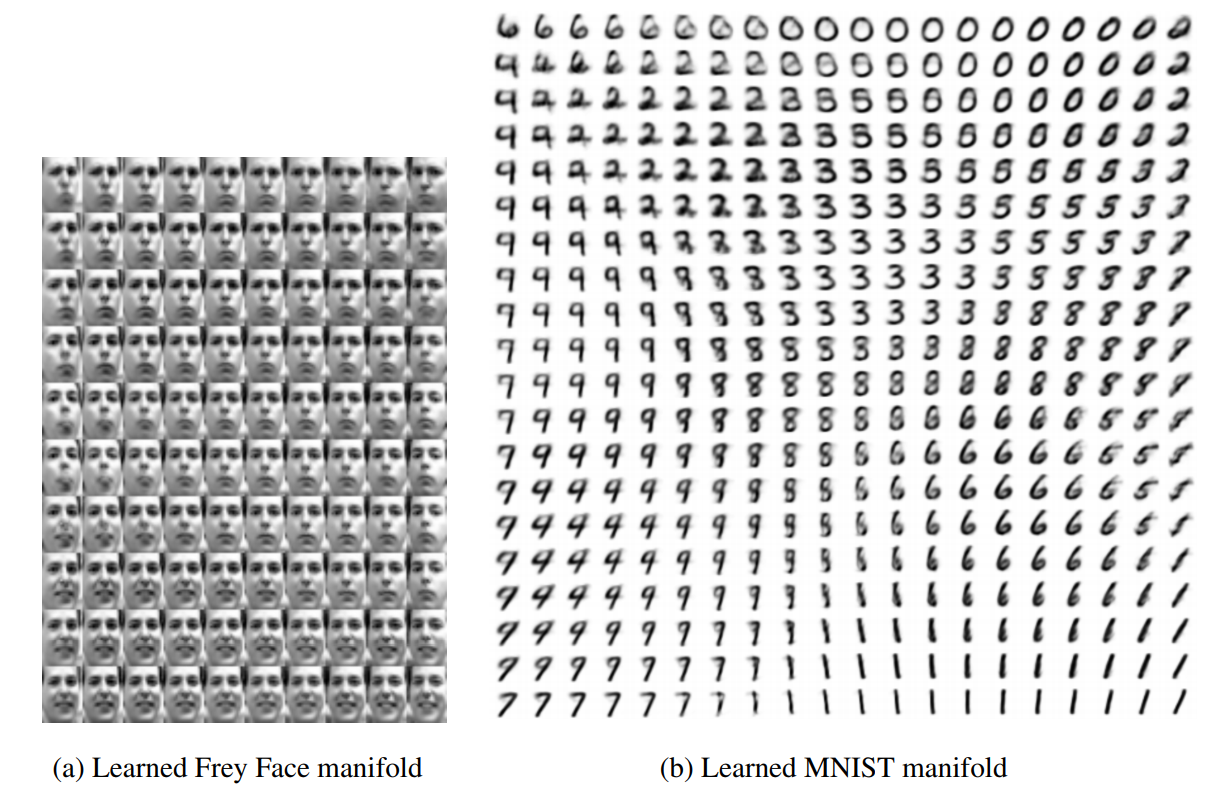
\includegraphics[width=1\textwidth]{imgs/vae_freyface_mnist.png}
                \caption{Figure by \cite{kingma2013auto} which shows the generated images from the latent values traversed uniformly across the 2D latent space.}
                \label{fig:vae_freyface_mnist}
            \end{figure}

            As we can see in the figure \ref{fig:vae_freyface_mnist}, the continously interpolated images make intuitive sense. If we consider the MNIST generated images, we even have interpolations between two different digits which seem almost plausible.
            
            In fact, VAE also does well at producing latent spaces which satisfy the second condition of interpretability: disentangled representations. \cite{bengio2013representation} defined the disentangled representation as that which has the property such that changes in a single latent dimension changes a single generative factor whilst leaving other generative factors mostly unchanged. \cite{higgins2017beta} includes figures showing how much VAE's representations are disentangled compared to other models.
            
            \begin{figure}[H]
                \centering
                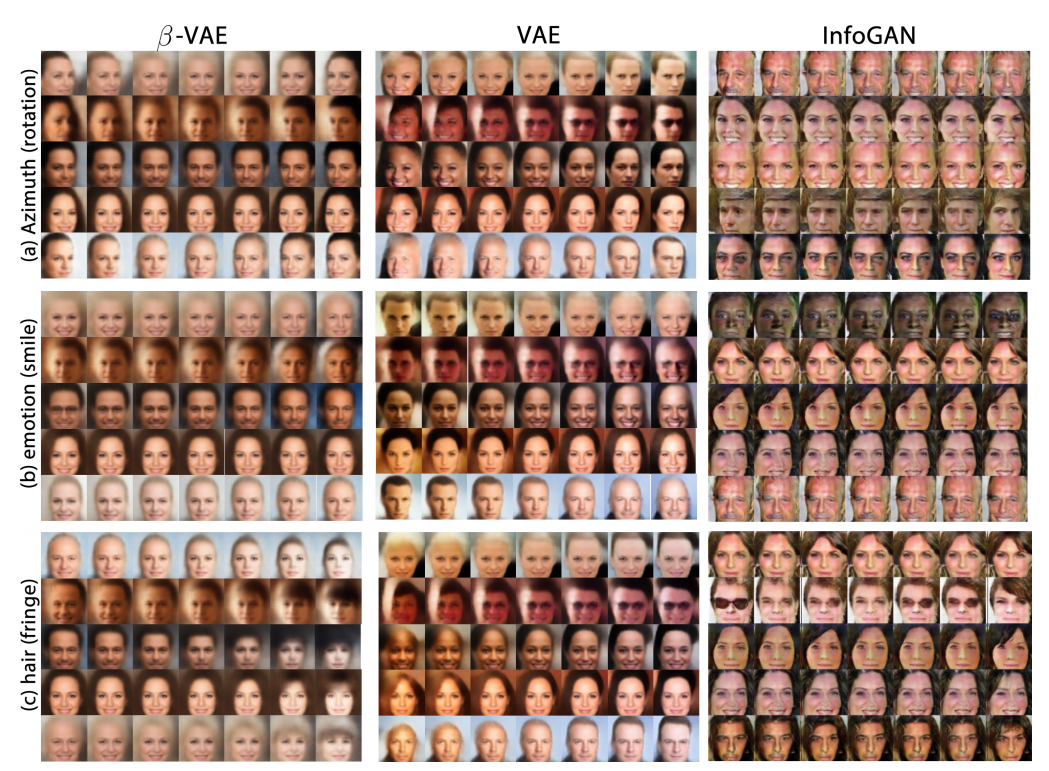
\includegraphics[width=1\textwidth]{imgs/celeba.png}
                \caption{Figures from \cite{higgins2017beta}. Qualitative comparison on disentanglement between $\beta$-VAE\citep{higgins2017beta}, VAE\citep{kingma2014adam}, and InfoGAN\citep{chen2016infogan} on images of celebrity faces.}
                \label{fig:celeba}
            \end{figure}    
            
            \begin{figure}[H]
                \centering
                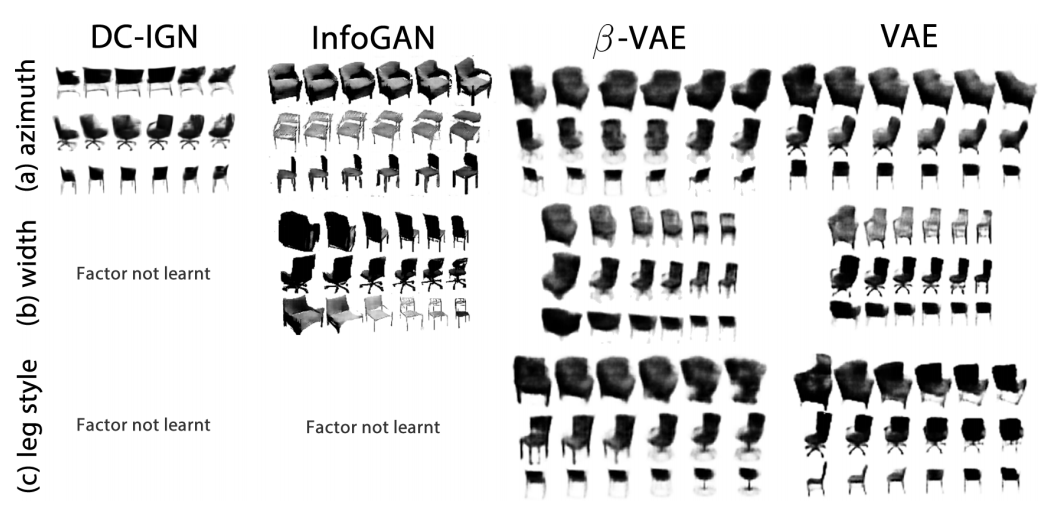
\includegraphics[width=1\textwidth]{imgs/3d_chairs.png}
                \caption{Figures from \cite{higgins2017beta}. Qualitative comparison on disentanglement between DC-IGN\citep{kulkarni2015deep}, InfoGAN\citep{chen2016infogan}, $\beta$-VAE\citep{higgins2017beta}, and VAE\citep{kingma2014adam} on 3D images of chairs.}
                \label{fig:3d_chairs}
            \end{figure}  
            
            \begin{figure}[H]
                \centering
                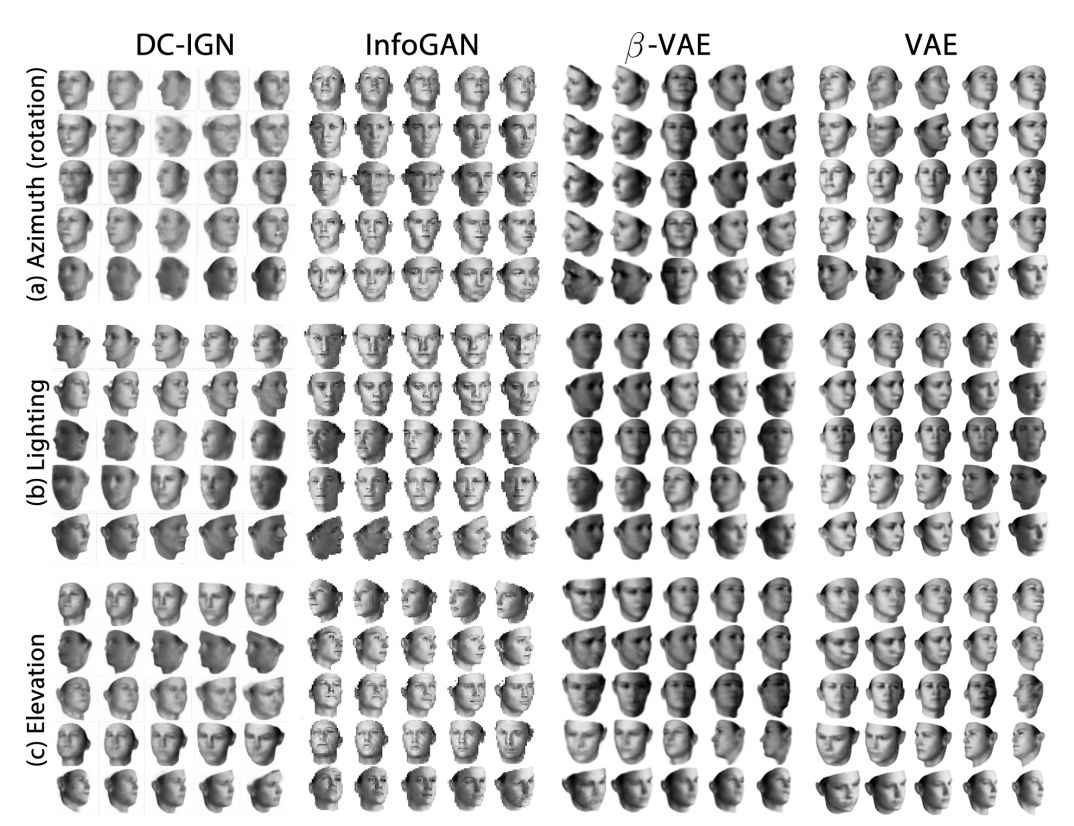
\includegraphics[width=1\textwidth]{imgs/3d_faces.png}
                \caption{Figures from \cite{higgins2017beta}. Qualitative comparison on disentanglement between DC-IGN\citep{kulkarni2015deep}, InfoGAN\citep{chen2016infogan}, $\beta$-VAE\citep{higgins2017beta}, and VAE\citep{kingma2014adam} on 3d images of faces.}
                \label{fig:3d_faces}
            \end{figure}  
            
            These figures show various input images acting as the seed and varying the value of a single latent dimension to show the change in a single generative factor. As we can see from the result images, VAE already does a good job at mapping some generative factors to single latent dimensions which is what is required for disentanglement. A more recent model called the $\beta$-VAE, expands on VAE and produces latent representations with better disentanglement.
            
    \section{Beta-Variational Autoencoder($\beta$-VAE)}
        \subsection{Model description}
            The $\beta$-VAE \citep{higgins2017beta} introduces a small modification to the original VAE. The only difference is the introduction of a single scalar $\beta$ as a hyperparameter in the original loss function. Recall that the loss function used in the original VAE is:
            
            \[ \text{Loss\textsubscript{VAE}} = \mathbb{E}_{q_{\bm{\theta_x}}(\bm{z}|\bm{x})} \left[\log p(\bm{x} | \bm{z}) \right] + KL\left[q_{\bm{\theta_x}}(\bm{z}|\bm{x}) || p(\bm{z})\right] \]
            
            The loss function for the $\beta$-VAE is:
            
            \[ \text{Loss\textsubscript{$\beta$-VAE}} = \mathbb{E}_{q_{\bm{\theta_x}}(\bm{z}|\bm{x})} \left[\log p(\bm{x} | \bm{z}) \right] + \textcolor{red}{\beta} KL\left[q_{\bm{\theta_x}}(\bm{z}|\bm{x}) || p(\bm{z})\right] \]
            
            By construction, $\beta=1$ gives the standard VAE but \cite{higgins2017beta} argues that the $\beta$-VAE, when $\beta>1$ improves disentanglement.
            
        \subsection{Intuitive reasoning behind the $\beta$-VAE} \label{subsec:beta_reasoning}
            Recall that we can interpret the original VAE's loss function as:
            
            \[ \text{Loss\textsubscript{VAE}} = \text{Reconstruction Loss} + \text{KL Divergence} \]
            
            Then the $\beta$-VAE's loss function can be interpreted as:
            
            \[ \text{Loss\textsubscript{$\beta$-VAE}} = \text{Reconstruction Loss} + \textcolor{red}{\beta} \text{ KL Divergence} \]
            
            This makes the intent behind placing a scalar in front of the KL divergence clear enough. It is to be able to control the weight the KL divergence has on the total loss function. By increasing the value of $\beta$, the model will prioritise keeping all the latent distributions as close to the prior distribution (i.e., the standard Gaussian). By decreasing the value of $\beta$, the model will prioritise improving the reconstruction accuracy. To get the gist of the effect this priority has, it is enough to see one example from our results from the project below. The exact setup and the details will be explained in the following chapters, but for now, we wish to illustrate a basic comparison.
            
            \begin{figure}[H]
                \centering
                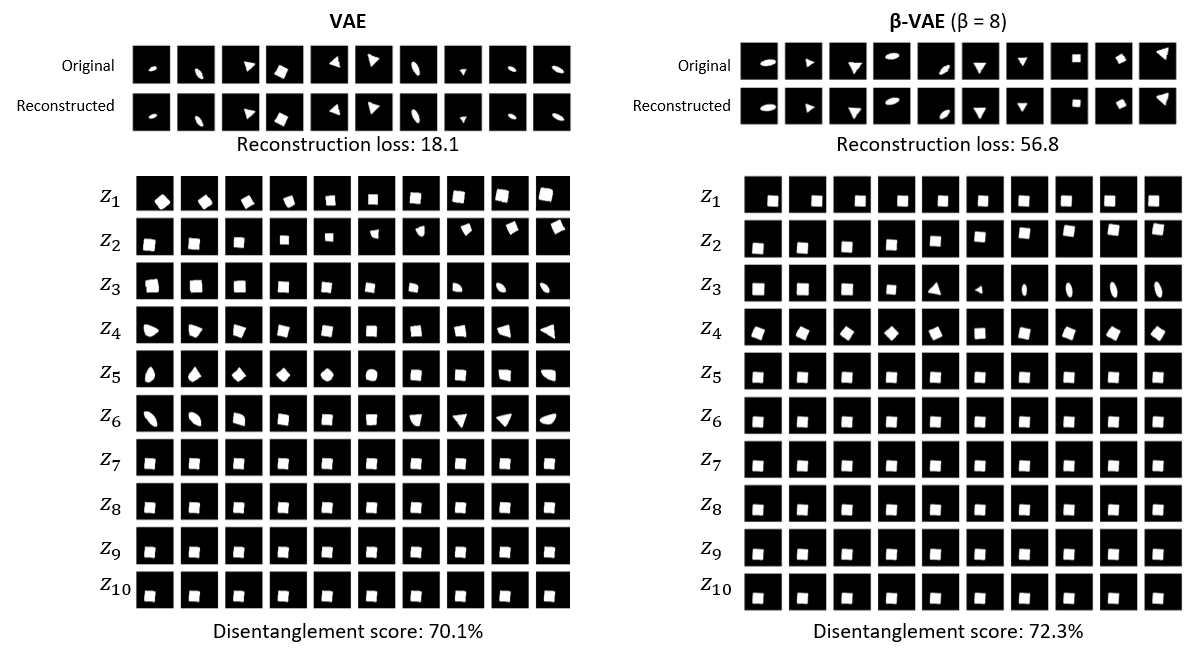
\includegraphics[width=1\textwidth]{imgs/entangled_disentangled.png}
                \caption{Example of entangled representations vs disentangled representations. Beginning with a seed of a single random input image which is encoded into the latent vectors, each row shows the generated images when we traverse through a single latent dimension from -3 to 3 standard deviations whilst keeping all others constant.}
                \label{fig:entangled_disentangled}
            \end{figure}  
            
            The above is an example of a clear illustration of the difference between a model which produced a relatively entangled representation of the input space and a model which produced a relatively disentangled representation of the input space.
            
            \begin{center}
                \begin{tabular}{| c || c | c | c | c | c |} 
                    \multicolumn{6}{c}{\textbf{VAE}} \\
                    \hline
                    & x-pos. & y-pos. & Scale & Shape & Ori. \\
                    \hline
                    $z_1$ & \checkmark & \checkmark & \checkmark & & \checkmark\\
                    \hline
                    $z_2$ & \checkmark & \checkmark & \checkmark & \checkmark & \checkmark\\
                    \hline
                    $z_3$ & & & \checkmark & \checkmark &\\
                    \hline
                    $z_4$ & & & & \checkmark & \checkmark\\
                    \hline
                    $z_5$ & & & & \checkmark & \checkmark\\
                    \hline
                    $z_6$ & & & & \checkmark &\\
                    \hline
                    $z_7$ & & & & &\\
                    \hline
                    $z_8$ & & & & &\\
                    \hline
                    $z_9$ & & & & &\\
                    \hline
                    $z_{10}$ & & & & &\\
                    \hline
                \end{tabular}
                \quad
                \begin{tabular}{| c || c | c | c | c | c |} 
                    \multicolumn{6}{c}{$\bm{\beta}$-\textbf{VAE}} \\
                    \hline
                    & x-pos. & y-pos. & Scale & Shape & Ori. \\
                    \hline
                    $z_1$ & \checkmark & & & &\\
                    \hline
                    $z_2$ & & \checkmark & & &\\
                    \hline
                    $z_3$ & & & \checkmark & \checkmark &\\
                    \hline
                    $z_4$ & & & & & \checkmark\\
                    \hline
                    $z_5$ & & & & &\\
                    \hline
                    $z_6$ & & & & &\\
                    \hline
                    $z_7$ & & & & &\\
                    \hline
                    $z_8$ & & & & &\\
                    \hline
                    $z_9$ & & & & &\\
                    \hline
                    $z_{10}$ & & & & &\\
                    \hline
                \end{tabular}
            \end{center}
            
            We can clearly see that the standard VAE is representing more than one feature per dimension and that features are represented across many dimensions. It is a many to many mapping which result in entangled representations. On the other hand, the $\beta$-VAE's($\beta=8$) mapping is nearly one-to-one which results in more disentangled representations.
            
            In some situations, the standard KL divergence may not provide a strong enough incentive to encode the latent space in the most information efficient way, instead focusing on reconstruction loss. This was exactly the case with the example above since the standard VAE produced better reconstructions than that of $\beta$-VAE. Indeed, most of the time, the value of the reconstruction loss is much bigger in magnitude than the value of the KL divergence. Therefore, it intuitively makes sense to adjust the weight that the KL divergence has on the total loss with the hope that a stronger weight on the KL divergence will produce a latent space which has better disentanglement.
            
            However, there is yet to be a formal argument as to why this should improve disentanglement. \cite{burgess2018understanding}) offers an intuitive explanation based on the argument that the $\beta$-VAE loss function is closely related to the \textit{information bottleneck principle} (\cite{tishby2000information}, \cite{achille2018information}, \cite{alemi2016deep}, \cite{chechik2005information}):
                \[\text{max}[I(Z;Y) - \beta I(X;Z)]\]
            where $I(\cdot; \cdot)$ stands for mutual information and $\beta$ is a Lagrange multiplier. Optimising the above objective requires maximising the mutual information shared between the latent bottleneck $Z$ and the given task $Y$ whilst at the same time trying to remove all information $Y$ shared by $X$. \cite{burgess2018understanding} explains that we can see the posterior $q_{\bm{\theta_x}}(\bm{z}|\bm{x})$ as the information bottleneck $Z$, and the reconstruction objective $\mathbb{E}_{q_{\bm{\theta_x}}(\bm{z}|\bm{x})} \left[\log p(\bm{x} | \bm{z}) \right]$ as the task $Y$ which encourages the latent distribution $q_{\bm{\theta_x}}(\bm{z}|\bm{x})$ to \textit{efficiently} represent the input $\bm{x}$ by jointly minimising the reconstruction loss and the $\beta$-weighted KL divergence. In the information theoretic perspective, the KL divergence can be seen as an upper bound on the amount of information that can be transmitted through the latent channels per data sample.
            
            \cite{burgess2018understanding} continues to explain that the KL divergence encourages the embedding of the input space to have the property that points close in the input space are mapped to points close in the latent space. This is because to minimise the KL divergence between the posterior uncorrelated multivariate Gaussian and the prior standard multivariate Gaussian, the posterior Gaussian needs to do two things. First, the posterior mean values need to stay close to zero against the model's tendency to freely vary the mean values to best represent data. Secondly, the posterior standard deviations need to stay close to one against the model's tendency to have vary small standard deviations to partition the input space into as many small parts as possible which will decrease the reconstruction loss at the cost of losing the continuity in the latent space.
            
            Now bearing in mind these two properties, consider the diagrams below. Each Gaussian distribution below represents the posterior distribution with respect to the input shown above as an example. We will illustrate the important role the KL divergence has and furthermore, the significance the \textit{weight} of the KL divergence will have in the training.
            
            \begin{figure}[H]
                \centering
                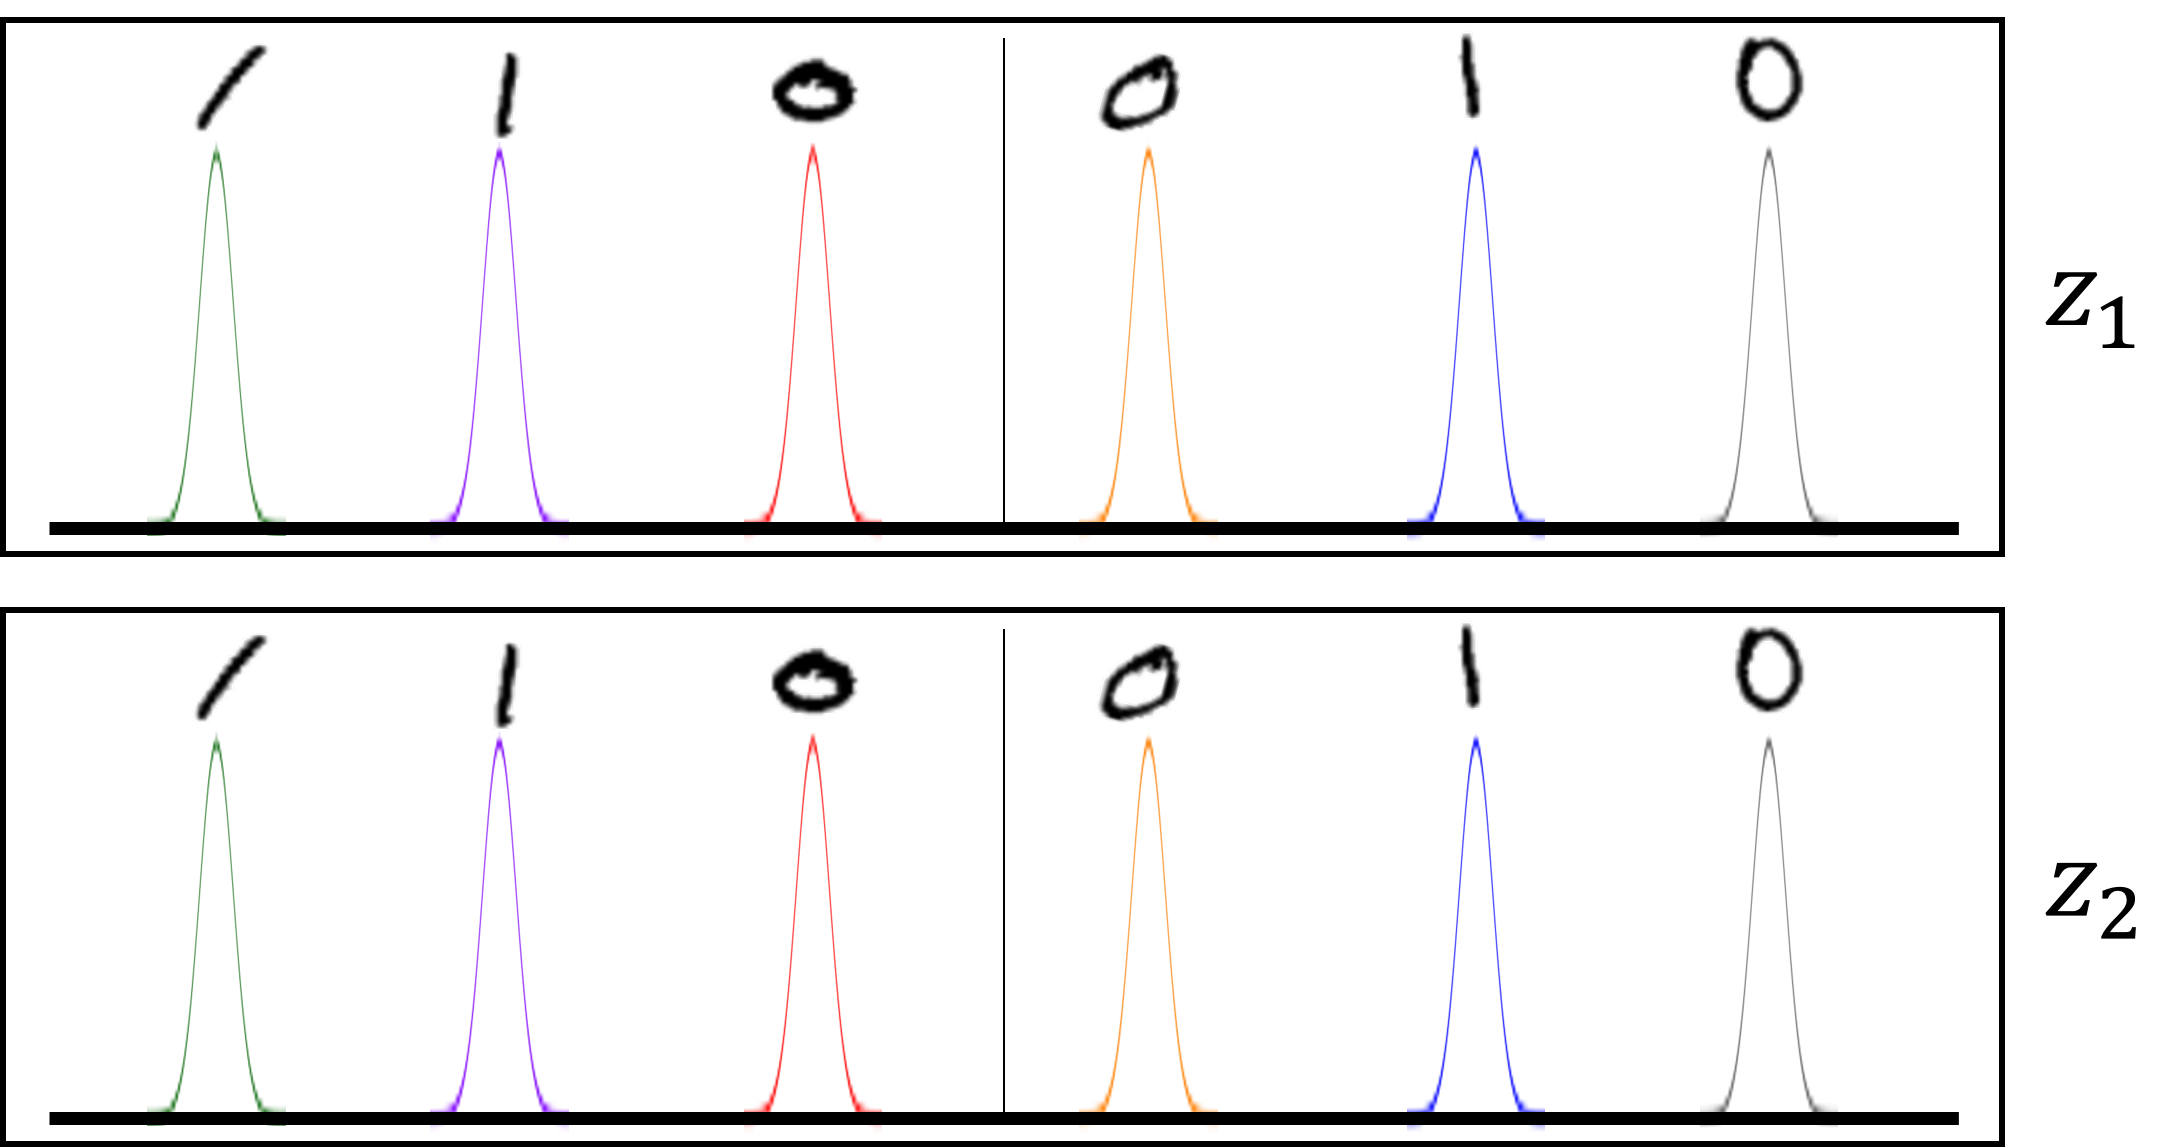
\includegraphics[width=0.5\textwidth]{imgs/1d_beta_size1.png}
                \caption{Posterior distributions with no KL divergence.}
                \label{fig:1d_beta_size1}
            \end{figure}
            
            Figure \ref{fig:1d_beta_size1} shows the kind of distributions we should expect to see if the final objective does not include the KL divergence. The reconstruction loss is maximised if the model "memorises" the input space by mapping distinct latent distribution for each input data point. As discussed in the previous section, this is undesirable outcome as the model will not produce an interpretable latent space.
            
            \begin{figure}[H]
                \centering
                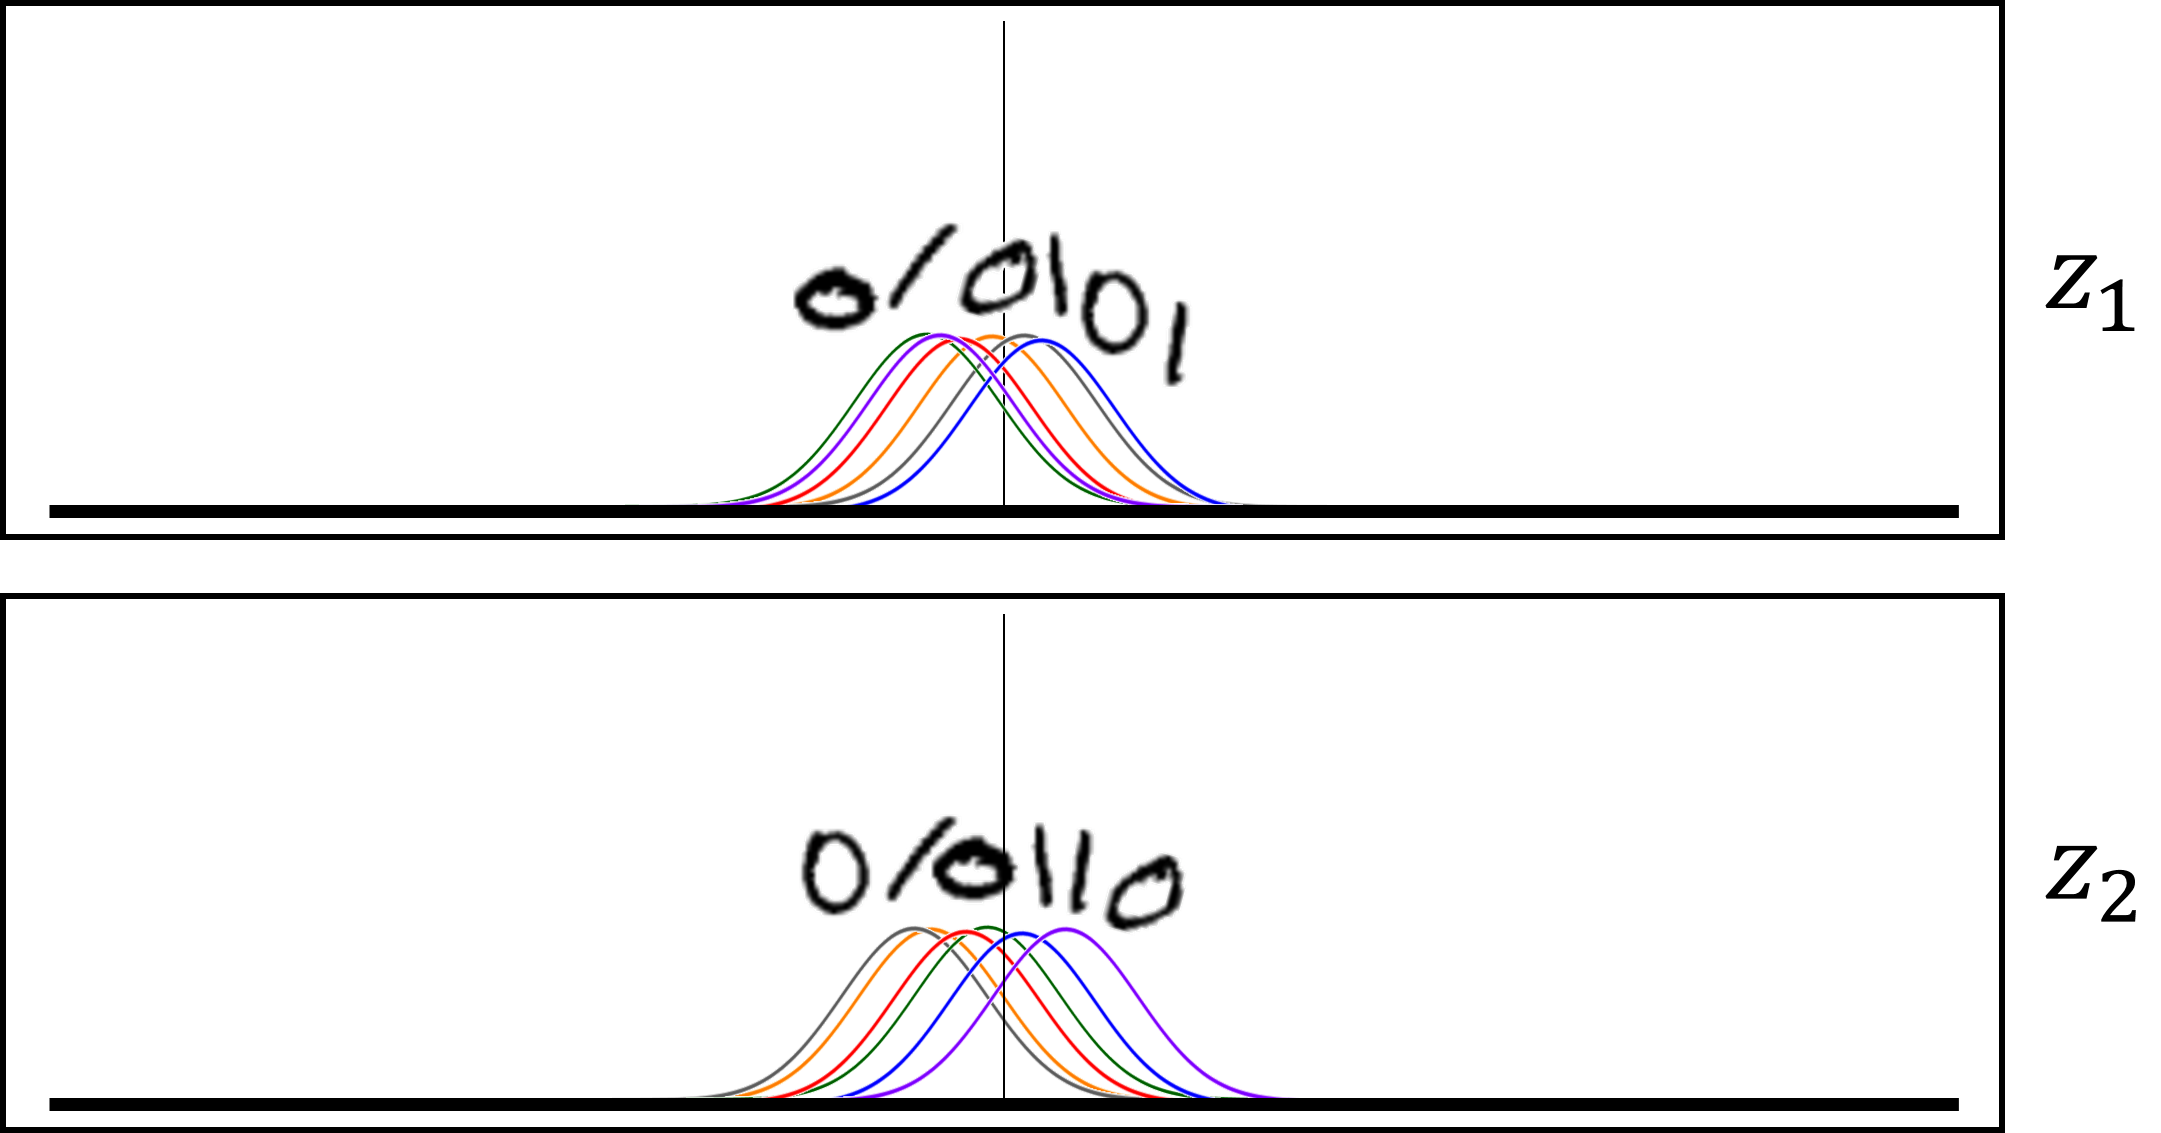
\includegraphics[width=0.5\textwidth]{imgs/1d_beta_size2.png}
                \caption{Posterior distributions with too much weight on the KL divergence.}
                \label{fig:1d_beta_size2}
            \end{figure}
            
            Figure \ref{fig:1d_beta_size2} shows the kind of distributions we should expect to see if the final objective includes too much weight on the KL divergence. Since the KL divergence encourages all the posterior distributions to have zero mean and 1 standard deviation, if we give too much weight on the KL divergence, all the distributions will overlap as the standard Gaussian and will give a blurry output as an average between all the input points which is also a problem.
            
            \begin{figure}[H]
                \centering
                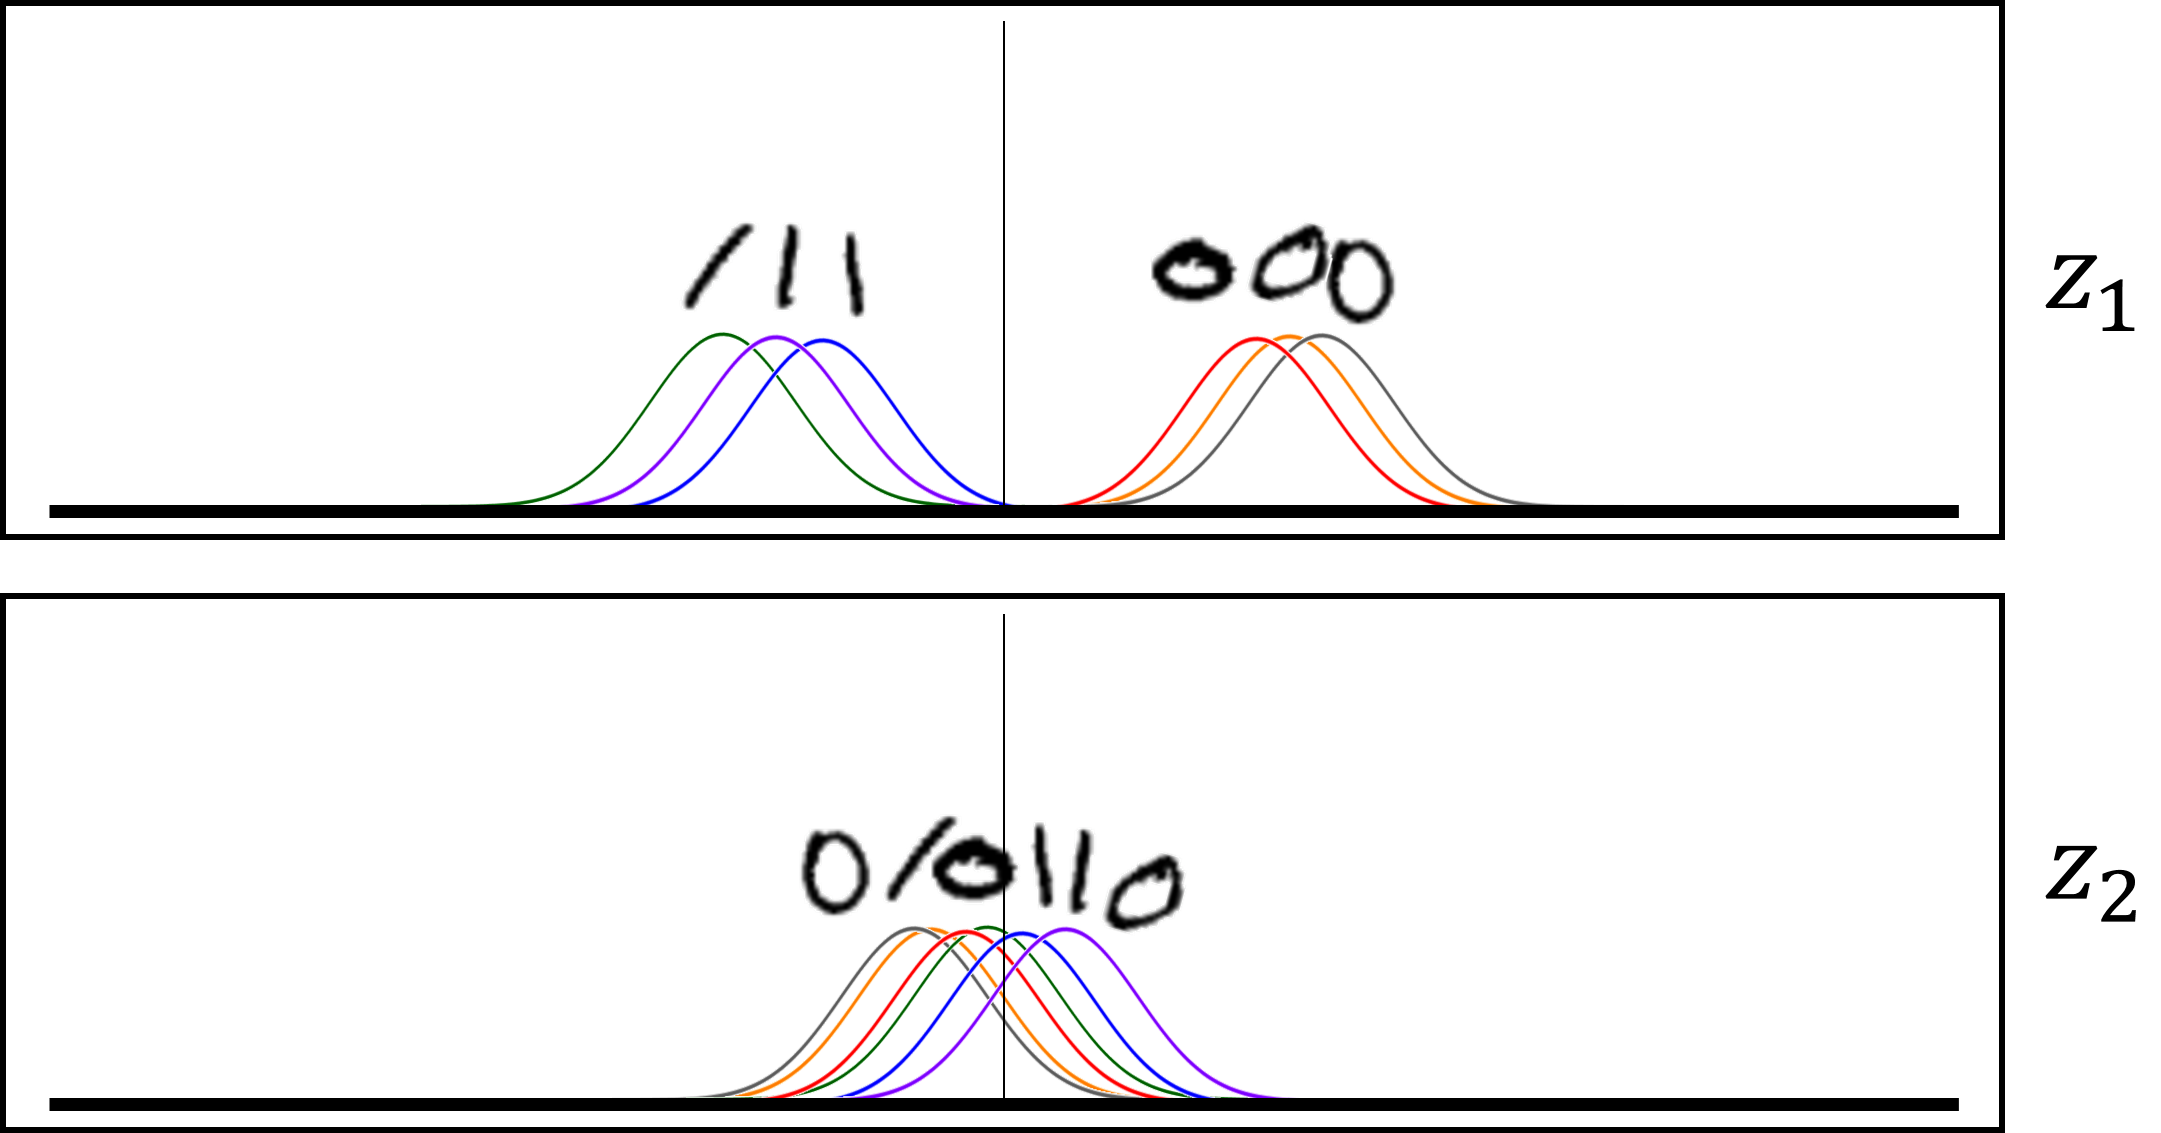
\includegraphics[width=0.5\textwidth]{imgs/1d_beta_size3.png}
                \caption{Posterior distributions with a relatively large weight on the KL divergence.}
                \label{fig:1d_beta_size3}
            \end{figure}
            
            Figure \ref{fig:1d_beta_size3} shows the kind of distributions we should expect to see if the final objective includes a relatively large weight on the KL divergence. The first latent dimension $z_1$ has learnt to discriminate between the digits. It was able to do this because the KL divergence encourages a large standard deviation and the mean values to be as close to 1 as possible. The model has learned to compromise between the reconstruction loss and the KL divergence by mapping similar input points near each other so that even if the model mistakenly samples a latent value from the "wrong" overlapping distribution, the output will not deviate much from the actual input. However, the large weight on the KL divergence means that the reconstruction gain from learning any other features through the second dimension was not worth the increase in the KL divergence by transforming the standard Gaussians. This model is much better than the previous two extremes but ideally, we would like to see it learn other minor but significant features such as slant.
            
            \begin{figure}[H]
                \centering
                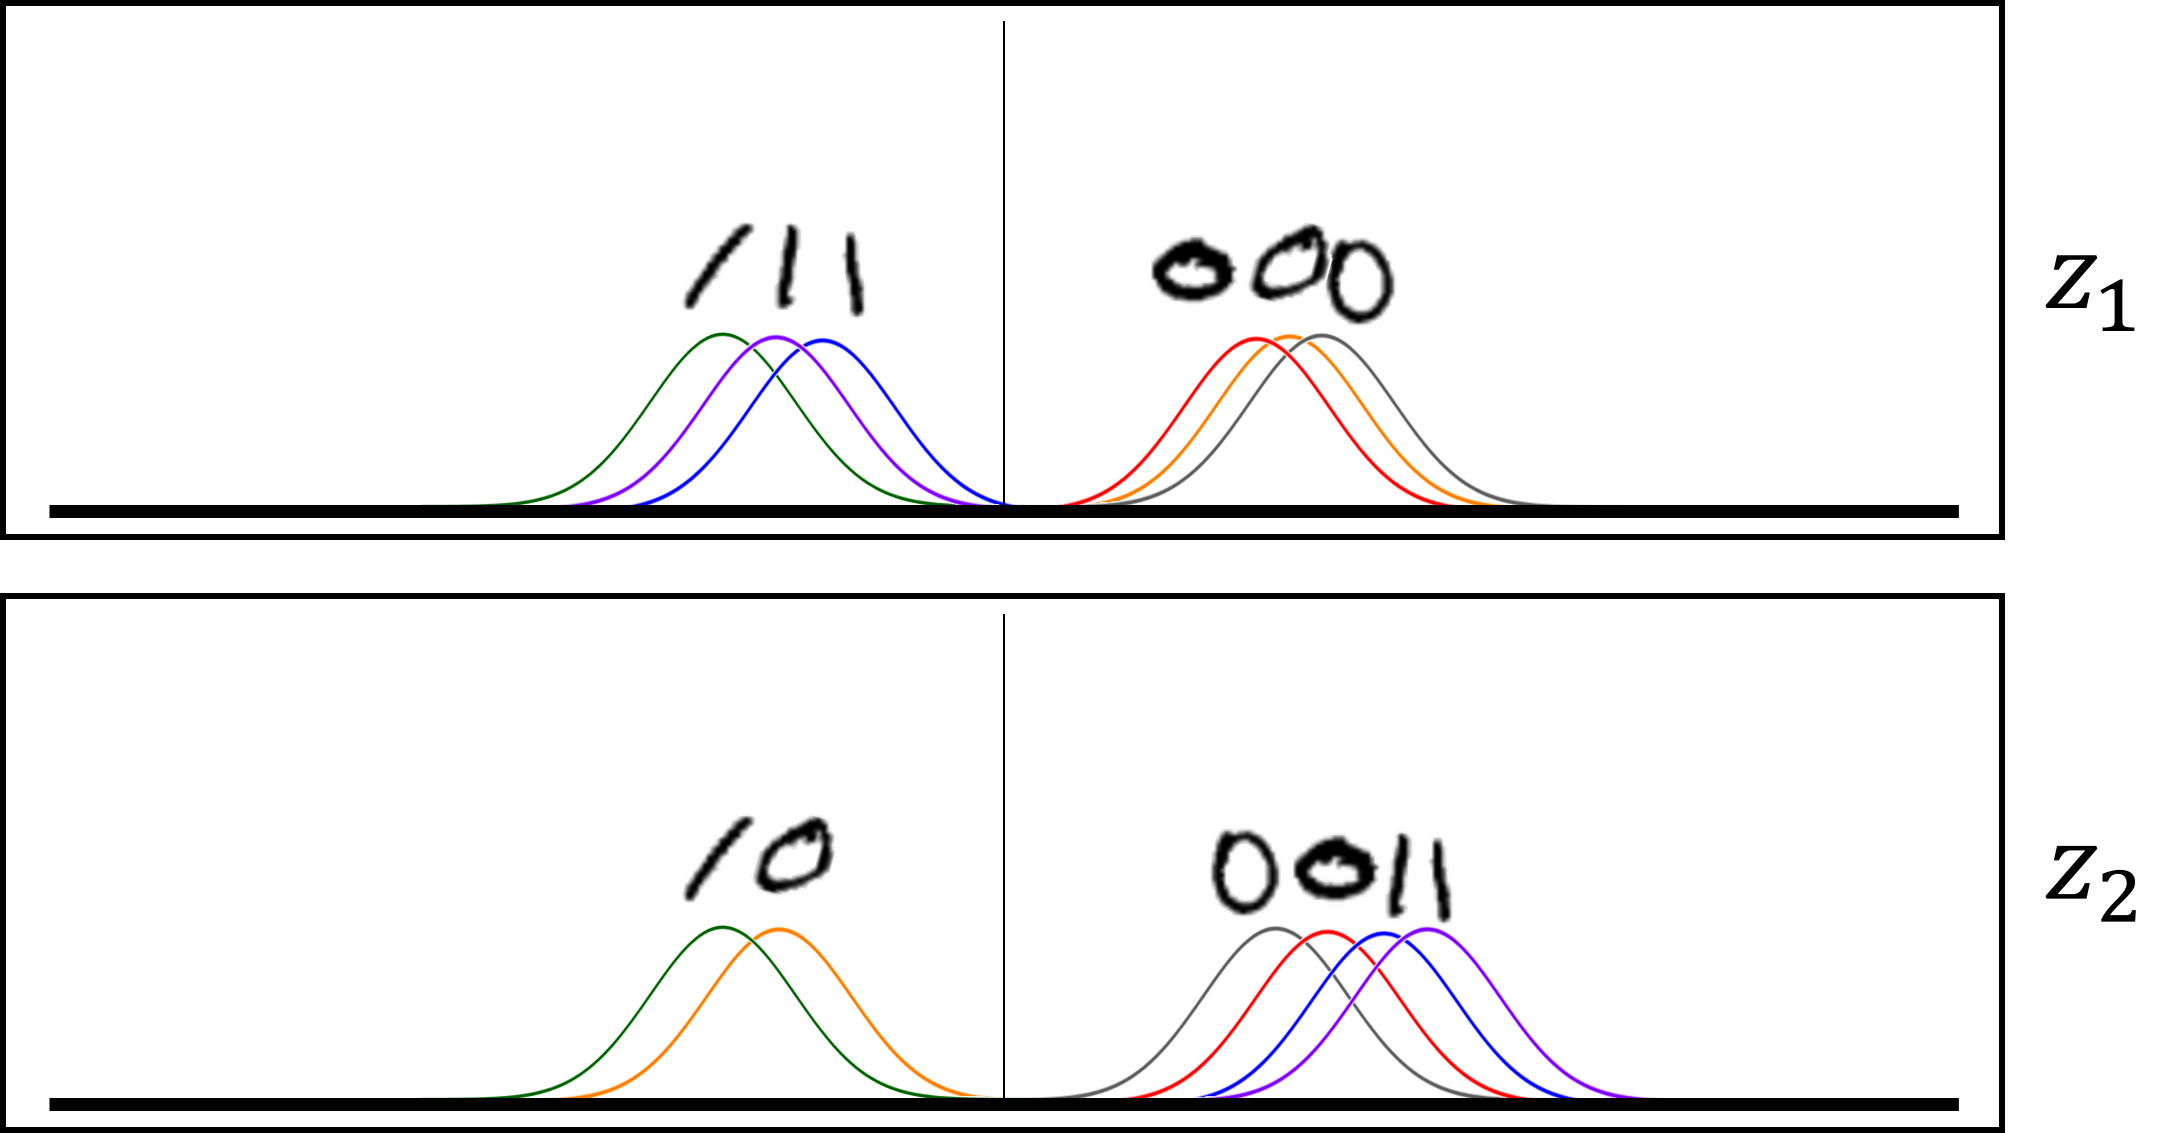
\includegraphics[width=0.5\textwidth]{imgs/1d_beta_size4.png}
                \caption{Posterior distributions with the optimal weight on the KL divergence.}
                \label{fig:1d_beta_size4}
            \end{figure}
            
            Figure \ref{fig:1d_beta_size4} shows the kind of distributions we should expect to see if the final objective includes an optimum weight on the KL divergence. The first latent dimension $z_1$ has learnt to discriminate between the digits as with the figure before. Now with a slightly smaller weight on the KL divergence, the second dimension had just the right amount of capacity to learn another feature(the slant in this case) at the cost of increasing the KL divergence but with the gain of less reconstruction loss. This is the ideal model which is the right balance between the reconstruction loss(how accurately we can retrieve the original input) and the KL divergence(interpretability).
            
            In this perspective, it makes sense to put a hyperparameter $\beta$ to give a weight on the KL divergence for the total function. There is no reason to think that $\beta=1$ as in the case of the standard VAE will always be the optimal balance between the reconstruction and the KL divergence.